%% PAPER 1 (draft from v4): wired transport cost of PQC in financial messaging. Radio -> paper3, mitigations/capacity -> paper2.
%% [NEW] = work still to be done (see ../PLAN.md).
\documentclass[preprint,12pt]{elsarticle}

\usepackage[T1]{fontenc}
\usepackage{lmodern}
\usepackage{amsmath,amssymb}
\usepackage{booktabs,array,graphicx,xcolor,tabularx}
\usepackage{microtype}
\usepackage{xspace}
\usepackage{tikz}
\usetikzlibrary{positioning,arrows.meta,fit,calc}
\usepackage[hidelinks]{hyperref}
\usepackage{url}
\Urlmuskip=0mu plus 2mu\relax
\def\UrlBreaks{\do\/\do\-\do\.}
\usepackage[capitalise,nameinlink]{cleveref}
\usepackage{caption}
\usepackage[section]{placeins}
% Revision highlights: set \highlightchangesfalse for the submission version (changes then print as plain text and soul is not loaded).
\newif\ifhighlightchanges\highlightchangesfalse
\ifhighlightchanges\usepackage{soul}\newcommand{\chg}[1]{{\sethlcolor{yellow}\hl{#1}}}\else\newcommand{\chg}[1]{#1}\fi
\captionsetup{font=small,labelfont=bf}
\setlength{\emergencystretch}{2em}

% Generated by make_assets.py - do not edit
\newcommand{\absPenQuic}{106}
\newcommand{\absPenTcp}{105}
\newcommand{\appDeltaErr}{4.1}
\newcommand{\appDpopEC}{518}
\newcommand{\appDpopML}{8{,}206}
\newcommand{\appXmlErr}{0.7}
\newcommand{\baseSixHi}{141}
\newcommand{\baseSixLo}{397}
\newcommand{\baseSwiftMs}{121.5}
\newcommand{\beML}{0.08}
\newcommand{\beMLmbs}{13}
\newcommand{\beRSA}{1.70}
\newcommand{\beSLHf}{0.02}
\newcommand{\blerSixHi}{9}
\newcommand{\blerSixLo}{12}
\newcommand{\busyWarmBase}{31}
\newcommand{\busyWarmML}{34}
\newcommand{\capEC}{15{,}129}
\newcommand{\capHyb}{11{,}614}
\newcommand{\capHybPct}{30}
\newcommand{\capML}{2{,}845}
\newcommand{\capMLm}{2{,}012}
\newcommand{\capMLratio}{5.3}
\newcommand{\ccMatHi}{21}
\newcommand{\ccMatLo}{5}
\newcommand{\ccMaxRttML}{1.00}
\newcommand{\ccRedEC}{31}
\newcommand{\ccRedFal}{12}
\newcommand{\ccRedML}{5}
\newcommand{\ccRedRSA}{22}
\newcommand{\ccRedSLHf}{2}
\newcommand{\certErrMax}{0.8}
\newcommand{\ciMLHi}{3.86}
\newcommand{\ciMLLo}{3.85}
\newcommand{\ciMaxHalf}{15.7}
\newcommand{\compErrPQ}{5}
\newcommand{\compRealECfour}{0.40}
\newcommand{\compRealPQhi}{0.98}
\newcommand{\compRealPQlo}{0.88}
\newcommand{\compositeDepthDelta}{60.4}
\newcommand{\compositeDepthDeltaIdeal}{32.8}
\newcommand{\compositeExtraPct}{0.3}
\newcommand{\desFlows}{126{,}360}
\newcommand{\desMaxDiff}{1.3\times10^{-11}}
\newcommand{\dlFrHi}{2.3}
\newcommand{\dlSixHi}{411}
\newcommand{\dlSixLo}{2.5}
\newcommand{\dlThzHi}{4.3}
\newcommand{\dlUrHi}{42}
\newcommand{\ecCpuMs}{0.5}
\newcommand{\ecDepthDelta}{29.6}
\newcommand{\ecDepthDeltaIdeal}{0.6}
\newcommand{\effSlowdown}{2.0}
\newcommand{\falDepthDelta}{1.2}
\newcommand{\falDepthPen}{0}
\newcommand{\falSignMeas}{0.10}
\newcommand{\falSwiftMs}{123.1}
\newcommand{\fullSfML}{16{,}841}
\newcommand{\harmEmbEC}{0}
\newcommand{\harmEmbML}{95}
\newcommand{\harmEmbRSA}{31}
\newcommand{\harmEmbSLHf}{100}
\newcommand{\harmSrvEC}{0}
\newcommand{\harmSrvML}{0}
\newcommand{\harmSrvRSA}{0}
\newcommand{\harmSrvSLHf}{0}
\newcommand{\hsResidHi}{1.1}
\newcommand{\hsResidLo}{-0.1}
\newcommand{\hybDepthDelta}{29.6}
\newcommand{\hybKneeBase}{121}
\newcommand{\hybKneeBaseIdeal}{121}
\newcommand{\hybKneeHyb}{122}
\newcommand{\hybKneeHybIdeal}{92}
\newcommand{\hybridDeltaKB}{2.2}
\newcommand{\hybridDeltaMs}{0.2}
\newcommand{\icwTenECdOne}{92.1}
\newcommand{\icwTenMLdOne}{127.3}
\newcommand{\icwThirtyTwoECdOne}{92.1}
\newcommand{\icwThirtyTwoMLDelta}{29.9}
\newcommand{\icwThirtyTwoMLdOne}{98.2}
\newcommand{\idleWarmML}{92}
\newcommand{\inetCf}{2.9}
\newcommand{\inetCfHi}{4.4}
\newcommand{\inetCfLo}{1.2}
\newcommand{\inetCfRtt}{30}
\newcommand{\inetGg}{2.5}
\newcommand{\inetGgHi}{5.7}
\newcommand{\inetGgLo}{0.1}
\newcommand{\inetGgRtt}{34}
\newcommand{\inetN}{400}
\newcommand{\lossFactorTwo}{1.71}
\newcommand{\lossFactorZero}{1.69}
\newcommand{\lossGapTwo}{144}
\newcommand{\lossGapZero}{105}
\newcommand{\lossSlhGapTwo}{474}
\newcommand{\lossThzLo}{0.81}
\newcommand{\meanMmBase}{169}
\newcommand{\metaLargeECDelta}{1}
\newcommand{\mitCiRadioHi}{1.29}
\newcommand{\mitCiRadioLo}{3.75}
\newcommand{\mitCiShare}{66}
\newcommand{\mitCiWired}{1.45}
\newcommand{\mitMtcRadioHi}{1.29}
\newcommand{\mitMtcRadioLo}{3.76}
\newcommand{\mitMtcShare}{54}
\newcommand{\mitMtcWired}{1.49}
\newcommand{\mitNoneRadioHi}{1.49}
\newcommand{\mitNoneRadioLo}{3.85}
\newcommand{\mitNoneWired}{1.69}
\newcommand{\mitQuicResWired}{1.13}
\newcommand{\mitQuicSaveMs}{30}
\newcommand{\mitQuicWired}{1.50}
\newcommand{\mitResRadioHi}{1.11}
\newcommand{\mitResRadioLo}{3.18}
\newcommand{\mitResWired}{1.33}
\newcommand{\mlCpuMs}{3.4}
\newcommand{\mlDepthCpu}{0.6}
\newcommand{\mlDepthDelta}{60.0}
\newcommand{\mlDepthDeltaEightSeven}{32.3}
\newcommand{\mlDepthDeltaEightSevenIdeal}{32.1}
\newcommand{\mlDepthDeltaIdeal}{59.9}
\newcommand{\mlDepthNet}{30.5}
\newcommand{\mlDepthSer}{2.9}
\newcommand{\mlDepthSsw}{56.5}
\newcommand{\mlSixHi}{210}
\newcommand{\mlSixLo}{1531}
\newcommand{\mlSswFirstDepth}{1}
\newcommand{\mlSwiftMs}{186.1}
\newcommand{\mldsaSignOqs}{0.27}
\newcommand{\mldsaSignOssl}{0.59}
\newcommand{\mldsaSignVone}{0.22}
\newcommand{\nCold}{140{,}400}
\newcommand{\nConfigs}{175{,}500}
\newcommand{\nRadioRows}{5{,}460}
\newcommand{\nRadioTx}{5{,}460{,}000}
\newcommand{\nTrials}{1{,}000}
\newcommand{\nocertMLKB}{67.2}
\newcommand{\nocertWarmML}{33}
\newcommand{\pNineNineMmBase}{1026}
\newcommand{\perCertNet}{10.2}
\newcommand{\perCertNineZeroZeroZeropTwoFour}{9.1}
\newcommand{\perCertNineZeroZeroZeropZero}{1.1}
\newcommand{\perCertOneFiveZeroZeropTwoFour}{20.0}
\newcommand{\perCertOneFiveZeroZeropZero}{20.0}
\newcommand{\perCertOneTwoEightZeropTwoFour}{10.5}
\newcommand{\perCertOneTwoEightZeropZero}{10.5}
\newcommand{\perCertRttFive}{3.3}
\newcommand{\perCertRttOneZeroZero}{66.7}
\newcommand{\quicGateTen}{0.5}
\newcommand{\quicGateThirtyTwo}{30}
\newcommand{\radDepthFourHi}{1.52}
\newcommand{\radDepthFourZero}{3.47}
\newcommand{\radDepthOneHi}{1.12}
\newcommand{\radDepthOneZero}{2.86}
\newcommand{\ratioECHundred}{57.1}
\newcommand{\ratioMLhundred}{27}
\newcommand{\ratioSLHsHundred}{0.1}
\newcommand{\resChML}{7{,}849}
\newcommand{\resSfML}{1{,}297}
\newcommand{\resTicketBase}{208}
\newcommand{\resTicketML}{6{,}352}
\newcommand{\retxSixLo}{1.04}
\newcommand{\rfFrhi}{1.46}
\newcommand{\rfFrlo}{2.16}
\newcommand{\rfFrzero}{1.76}
\newcommand{\rfMmhi}{1.38}
\newcommand{\rfMmlo}{2.39}
\newcommand{\rfMmzero}{2.14}
\newcommand{\rfSixFalLo}{1.76}
\newcommand{\rfSixHybHi}{1.00}
\newcommand{\rfSixHybLo}{1.10}
\newcommand{\rfSixSlhfHi}{2.5}
\newcommand{\rfSixSlhfLo}{11.9}
\newcommand{\rfSixhi}{1.49}
\newcommand{\rfSixlo}{3.86}
\newcommand{\rfSixzero}{3.11}
\newcommand{\rfThzhi}{1.39}
\newcommand{\rfThzlo}{2.08}
\newcommand{\rfThzzero}{1.53}
\newcommand{\rfUrllchi}{1.55}
\newcommand{\rfUrllclo}{4.44}
\newcommand{\rfUrllczero}{4.08}
\newcommand{\rlcMmLo}{42}
\newcommand{\rlcSixLo}{2.5}
\newcommand{\rsaDepthDelta}{0.6}
\newcommand{\seMax}{16}
\newcommand{\seMedian}{0.8}
\newcommand{\shareECxFour}{36}
\newcommand{\shareECxOne}{51}
\newcommand{\shareECxOneSix}{27}
\newcommand{\shareFalxFour}{65}
\newcommand{\shareFalxOne}{80}
\newcommand{\shareFalxOneSix}{52}
\newcommand{\shareMLxFour}{76}
\newcommand{\shareMLxOne}{87}
\newcommand{\shareMLxOneIdeal}{80}
\newcommand{\shareMLxOneSix}{50}
\newcommand{\shareRSAxFour}{35}
\newcommand{\shareRSAxOne}{45}
\newcommand{\shareRSAxOneSix}{12}
\newcommand{\shareSLHfxFour}{46}
\newcommand{\shareSLHfxOne}{84}
\newcommand{\shareSLHfxOneSix}{3}
\newcommand{\shareSLHsxFour}{0}
\newcommand{\shareSLHsxOne}{0}
\newcommand{\shareSLHsxOneSix}{0}
\newcommand{\slaBaseSix}{-5}
\newcommand{\slaFalSix}{0}
\newcommand{\slaMLFr}{-5}
\newcommand{\slaMLSix}{10}
\newcommand{\slaMLUrllc}{15}
\newcommand{\slaSlhfSix}{20}
\newcommand{\slhfSwiftMs}{288}
\newcommand{\slhsCpuMs}{685}
\newcommand{\slhsSignMeas}{171}
\newcommand{\slhsSwiftMs}{871}
\newcommand{\sobolLatMtu}{0.18}
\newcommand{\sobolLatRtt}{0.59}
\newcommand{\sobolLatRttF}{0.20}
\newcommand{\sobolLatSuite}{0.28}
\newcommand{\sobolLatSuiteF}{0.16}
\newcommand{\sobolRadProf}{0.12}
\newcommand{\sobolRadProto}{0.15}
\newcommand{\sobolRadSinr}{0.14}
\newcommand{\sobolRadSuite}{0.23}
\newcommand{\swiftKBFalconFiveTwelve}{39.9}
\newcommand{\swiftKBFalconTenTwentyFour}{56.4}
\newcommand{\swiftKBHybrid}{25.2}
\newcommand{\swiftKBMLDSAeightyseven}{106.8}
\newcommand{\swiftKBMLDSAfortyfour}{66.3}
\newcommand{\swiftKBMLDSAsixtyfive}{83.4}
\newcommand{\swiftKBRSAtwo}{27.2}
\newcommand{\swiftKBSLHf}{246.7}
\newcommand{\swiftKBSLHs}{126.3}
\newcommand{\swiftKBbase}{23.0}
\newcommand{\swiftMLappShare}{30}
\newcommand{\swiftMLcertShare}{42}
\newcommand{\swiftMLcvShare}{8}
\newcommand{\swiftMLfixedShare}{17}
\newcommand{\swiftXFalconFiveTwelve}{1.7}
\newcommand{\swiftXFalconTenTwentyFour}{2.4}
\newcommand{\swiftXHybrid}{1.1}
\newcommand{\swiftXMLDSAeightyseven}{4.6}
\newcommand{\swiftXMLDSAfortyfour}{2.9}
\newcommand{\swiftXMLDSAsixtyfive}{3.6}
\newcommand{\swiftXRSAtwo}{1.2}
\newcommand{\swiftXSLHf}{10.7}
\newcommand{\swiftXSLHs}{5.5}
\newcommand{\tdCells}{864}
\newcommand{\tdFactorModel}{3.86}
\newcommand{\tdFactorTrace}{3.84}
\newcommand{\tdMeanMax}{4.1}
\newcommand{\tdMeanMed}{0.36}
\newcommand{\tdPNineNineMax}{18}
\newcommand{\tdPNineNineMed}{0.3}
\newcommand{\tdWiredMax}{6.9}
\newcommand{\tdWiredMed}{0.12}
\newcommand{\tlsConfigs}{56}
\newcommand{\tlsErrMax}{0.40}
\newcommand{\tlsErrMed}{0.02}
\newcommand{\urllcBler}{0.07}
\newcommand{\warmFapiLo}{3.62}
\newcommand{\warmMLisoEightFiveEightThree}{0.0}
\newcommand{\warmMLisoTwoZeroZeroTwoTwo}{61}
\newcommand{\warmSixHi}{1.15}
\newcommand{\warmSixLo}{3.62}
\newcommand{\warmXFAPITwo}{4.8}
\newcommand{\warmXIsoTwoZeroTwoTwo}{3.1}
\newcommand{\wiredFiveSixZero}{3.91}
\newcommand{\wiredSixtySixZero}{2.28}
\newcommand{\xFAPITwoFalconFiveTwelve}{2.2}
\newcommand{\xFAPITwoMLDSAsixtyfive}{5.7}
\newcommand{\xISOEightFiveEightThreeFalconFiveTwelve}{2.8}
\newcommand{\xISOEightFiveEightThreeMLDSAsixtyfive}{6.8}
\newcommand{\xISOTwoZeroZeroTwoTwoFalconFiveTwelve}{2.0}
\newcommand{\xISOTwoZeroZeroTwoTwoMLDSAsixtyfive}{4.4}
\newcommand{\xOAUTHTwoRFCSixSevenFourNineFalconFiveTwelve}{2.1}
\newcommand{\xOAUTHTwoRFCSixSevenFourNineMLDSAsixtyfive}{5.0}
\newcommand{\xOIDCFalconFiveTwelve}{2.2}
\newcommand{\xOIDCMLDSAsixtyfive}{5.1}
\newcommand{\xSWIFTMXFalconFiveTwelve}{1.7}
\newcommand{\xSWIFTMXMLDSAsixtyfive}{3.6}

% Generated by Measurements/testbed/paper_assets.py - do not edit
\newcommand{\tbNConfigs}{226}
\newcommand{\tbNTrans}{6{,}960}
\newcommand{\tbNSuites}{6}
\newcommand{\tbMaeIdeal}{4.70}
\newcommand{\tbBiasIdeal}{-3.50}
\newcommand{\tbMaxIdeal}{97.1}
\newcommand{\tbOffIdeal}{21}
\newcommand{\tbRelIdeal}{1.5}
\newcommand{\tbMaeLinux}{3.34}
\newcommand{\tbBiasLinux}{-1.98}
\newcommand{\tbMaxLinux}{95.4}
\newcommand{\tbOffLinux}{12}
\newcommand{\tbRelLinux}{1.3}
\newcommand{\tbMaeStack}{1.65}
\newcommand{\tbBiasStack}{+0.10}
\newcommand{\tbMaxStack}{5.4}
\newcommand{\tbOffStack}{4}
\newcommand{\tbRelStack}{1.2}
\newcommand{\tbOffIdealOne}{11}
\newcommand{\tbOffIdealMaxRtt}{1.9}
\newcommand{\tbWinMeas}{148.9}
\newcommand{\tbWinIdeal}{121.8}
\newcommand{\tbWinLinux}{150.7}
\newcommand{\tbSegMeas}{147.3}
\newcommand{\tbSegIdealMs}{91.9}
\newcommand{\tbSegStackMs}{150.4}
\newcommand{\tbMaxStackRtt}{3.9, 5.4, 3.8}
\newcommand{\tbOutN}{144}
\newcommand{\tbOutMaeIdeal}{4.32}
\newcommand{\tbOutMaeStack}{2.04}
\newcommand{\tbOutMax}{5.4}
\newcommand{\tbOutOffIdeal}{11}
\newcommand{\tbOutOffStack}{0}
\newcommand{\tbOutBiasLow}{+1.1}
\newcommand{\tbOutBiasHigh}{-1.2}
\newcommand{\tbWithinOne}{110}
\newcommand{\tbInCi}{46}
\newcommand{\tbSizeLo}{0.95}
\newcommand{\tbSizeHi}{1.09}
\newcommand{\tbRttLo}{5}
\newcommand{\tbRttHi}{100}
\newcommand{\tbRates}{10, 100, 1000}
\newcommand{\tbMtus}{1280, 1500, 9000}
\newcommand{\tbIcws}{10, 32}
\newcommand{\tbSegExact}{237}
\newcommand{\tbSegTotal}{300}
\newcommand{\tbSegIdealExact}{78}
\newcommand{\tbRmseZeroPi}{2.16}
\newcommand{\tbPiFit}{0.00}
\newcommand{\tbThetaFit}{1}
\newcommand{\tbRmseBestPi}{2.16}
\newcommand{\tbKneeHyb}{121.2}
\newcommand{\tbKneeHybModel}{120.9}
\newcommand{\tbKneeBase}{121.0}
\newcommand{\tbKneeBaseModel}{120.7}
\newcommand{\tbCubicN}{216}
\newcommand{\tbCubicMae}{1.13}
\newcommand{\tbCubicOffIdeal}{19}
\newcommand{\tbCubicOffStack}{12}
\newcommand{\tbCubicBias}{+0.57}
\newcommand{\tbCubicMax}{4.9}
\newcommand{\tbProxyTcpN}{16}
\newcommand{\tbProxyTcpMean}{0.18}
\newcommand{\tbProxyTcpLo}{-0.22}
\newcommand{\tbProxyTcpHi}{0.31}
\newcommand{\tbProxyInspectN}{16}
\newcommand{\tbProxyInspectMean}{0.28}
\newcommand{\tbProxyInspectLo}{-0.50}
\newcommand{\tbProxyInspectHi}{0.55}

% Generated by Simulation/uncertainty.py - do not edit
\newcommand{\uMlFactorMed}{1.46}
\newcommand{\uMlFactorLo}{1.19}
\newcommand{\uMlFactorHi}{1.72}
\newcommand{\uFalFactorMed}{1.05}
\newcommand{\uFalFactorLo}{1.01}
\newcommand{\uFalFactorHi}{1.23}
\newcommand{\uMlPerCertMed}{20.5}
\newcommand{\uMlPerCertLo}{3.5}
\newcommand{\uMlPerCertHi}{27.9}
\newcommand{\uOverheadShare}{91}
\newcommand{\uOverheadLowCpu}{99}
\newcommand{\uOverheadHighCpu}{73}
\newcommand{\uOrderHolds}{100}
\newcommand{\uRhoCwndFactor}{-0.37}
\newcommand{\uRhoCwndPerCert}{-0.75}
\newcommand{\uRhoCpuFactor}{0.54}
\newcommand{\uRhoPenFactor}{0.47}
\newcommand{\uPerCertWTenMed}{22.5}
\newcommand{\uPerCertWTenLo}{20.1}
\newcommand{\uPerCertWTenHi}{28.4}
\newcommand{\uPerCertWThirtyTwoMed}{12.4}
\newcommand{\uPerCertWThirtyTwoLo}{10.1}
\newcommand{\uPerCertWThirtyTwoHi}{18.2}
\newcommand{\uPerCertWSixtyFourMed}{3.4}
\newcommand{\uPerCertWSixtyFourLo}{1.3}
\newcommand{\uPerCertWSixtyFourHi}{9.5}

% Generated by Measurements/x86/analyze_cpu_x86.py - do not edit
\newcommand{\cpuXSigMed}{3.15}
\newcommand{\cpuXSigMin}{1.7}
\newcommand{\cpuXSigMax}{8.06}
\newcommand{\cpuXKemMed}{3.87}
\newcommand{\cpuXKemMin}{2.24}
\newcommand{\cpuXKemMax}{4.35}
\newcommand{\cpuAArmMed}{2.1}
\newcommand{\cpuXMlSign}{2.93}
\newcommand{\cpuXEcSign}{2.78}
\newcommand{\cpuXFalSign}{3.45}
\newcommand{\cpuXSlhsSign}{7.71}
\newcommand{\cpuValN}{24}
\newcommand{\cpuValBias}{+1.14}
\newcommand{\cpuValMae}{1.52}
\newcommand{\cpuValRelMed}{39}
\newcommand{\cpuValResidMax}{4.82}
\newcommand{\cpuValRatioArm}{4.17}
\newcommand{\cpuShareEc}{38}
\newcommand{\cpuShareMl}{78}
\newcommand{\cpuShareFal}{66}
\newcommand{\cpuShareSlhs}{0}
\newcommand{\cpuShareSlhf}{19}
\newcommand{\cpuShareRsa}{42}

% Generated by Measurements/testbed/residual_analysis.py - do not edit
\newcommand{\resRmse}{2.16}
\newcommand{\resNmae}{1.2}
\newcommand{\resMaeLo}{1.48}
\newcommand{\resMaeHi}{1.83}
\newcommand{\resCoreN}{82}
\newcommand{\resCoreMae}{0.96}
\newcommand{\resAwayN}{144}
\newcommand{\resAwayMae}{2.04}
\newcommand{\resNmaeRttLo}{0.2}
\newcommand{\resNmaeRttHi}{4.9}
\newcommand{\resMaeRttLo}{0.92}
\newcommand{\resMaeRttHi}{1.84}
\newcommand{\resWorstErr}{5.4}
\newcommand{\resWorstSuite}{ML-DSA-65}
\newcommand{\resWorstRtt}{30}
\newcommand{\resWorstDepth}{2}
\newcommand{\resWorstMtu}{9000}
\newcommand{\resWorstIcw}{32}
\newcommand{\resUnderFive}{219}

% Generated by Measurements/testbed/analyze_variants.py - do not edit
\newcommand{\varCubicN}{216}
\newcommand{\varCubicMae}{1.13}
\newcommand{\varCubicMaeIdeal}{5.41}
\newcommand{\varCubicBias}{+0.57}
\newcommand{\varCubicMax}{4.9}
\newcommand{\varCubicOffStack}{12}
\newcommand{\varCubicOffIdeal}{19}
\newcommand{\varCubicPairs}{42}
\newcommand{\varCubicPairMed}{+0.07}
\newcommand{\varCubicPairMae}{0.24}
\newcommand{\varCubicPairMax}{0.7}
\newcommand{\varDelackN}{72}
\newcommand{\varDelackMae}{1.18}
\newcommand{\varDelackMaeIdeal}{11.06}
\newcommand{\varDelackBias}{+0.39}
\newcommand{\varDelackMax}{3.6}
\newcommand{\varDelackOffStack}{4}
\newcommand{\varDelackOffIdeal}{12}
\newcommand{\varDelackPairs}{42}
\newcommand{\varDelackPairMed}{+0.26}
\newcommand{\varDelackPairMae}{0.32}
\newcommand{\varDelackPairMax}{0.8}
\newcommand{\varTsN}{72}
\newcommand{\varTsMae}{1.25}
\newcommand{\varTsMaeIdeal}{11.04}
\newcommand{\varTsBias}{+0.40}
\newcommand{\varTsMax}{4.0}
\newcommand{\varTsOffStack}{6}
\newcommand{\varTsOffIdeal}{12}
\newcommand{\varTsPairs}{42}
\newcommand{\varTsPairMed}{+0.15}
\newcommand{\varTsPairMae}{0.30}
\newcommand{\varTsPairMax}{1.0}
\newcommand{\varDelackTsN}{72}
\newcommand{\varDelackTsMae}{1.26}
\newcommand{\varDelackTsMaeIdeal}{11.12}
\newcommand{\varDelackTsBias}{+0.48}
\newcommand{\varDelackTsMax}{3.6}
\newcommand{\varDelackTsOffStack}{8}
\newcommand{\varDelackTsOffIdeal}{14}
\newcommand{\varDelackTsPairs}{42}
\newcommand{\varDelackTsPairMed}{+0.12}
\newcommand{\varDelackTsPairMae}{0.31}
\newcommand{\varDelackTsPairMax}{1.5}
\newcommand{\varBbrN}{8}
\newcommand{\varBbrMae}{5.47}
\newcommand{\varBbrMaeIdeal}{5.51}
\newcommand{\varBbrBias}{-5.47}
\newcommand{\varBbrMax}{22.3}
\newcommand{\varBbrOffStack}{0}
\newcommand{\varBbrOffIdeal}{0}
\newcommand{\varBbrPairs}{8}
\newcommand{\varBbrPairMed}{+2.78}
\newcommand{\varBbrPairMae}{5.83}
\newcommand{\varBbrPairMax}{24.9}
\newcommand{\varPairMedMax}{0.3}
\newcommand{\varPairMaxAll}{1.5}
\newcommand{\varMaeMax}{1.26}
\newcommand{\varMaxLo}{3.6}
\newcommand{\varMaxHi}{4.9}

% Generated by Measurements/testbed/supp_paper1_extra.py - do not edit
\newcommand{\tickN}{40}
\newcommand{\tickSlowN}{6}
\newcommand{\tickSlowFrac}{0.51}
\newcommand{\tickMedDiff}{0.6}
\newcommand{\srvPqOvhMin}{1.18}
\newcommand{\srvPqOvhMax}{1.35}
\newcommand{\srvEcOvhMin}{1.8}
\newcommand{\srvEcOvhMax}{2.8}

\newcommand{\dB}{\,dB\xspace}
\newcommand{\ms}{\,ms\xspace}
\newcommand{\KB}{\,KB\xspace}
\newcommand{\MLDSA}{ML-DSA-65\xspace}
\newcommand{\supp}[1]{#1 of the Supplementary Material}


\journal{Computers \& Security}

\renewcommand{\topfraction}{0.9}\renewcommand{\textfraction}{0.08}\renewcommand{\floatpagefraction}{0.7}
\begin{document}
\begin{frontmatter}

\title{Beyond Message Size: How the Behaviour of Linux TCP and OpenSSL Turns Post-Quantum Signatures into Round Trips in Financial Messaging}


\author[a]{Trong-Hieu DINH\fnref{orc1}}
\ead{hieudt@hvnh.edu.vn}
\author[b]{Trong-Minh HOANG\corref{cor1}\fnref{orc2}}
\ead{hoangtrongminh@ptit.edu.vn}
\cortext[cor1]{Corresponding author}
\fntext[orc1]{ORCID: \href{https://orcid.org/0009-0005-0601-3229}{0009-0005-0601-3229}}
\fntext[orc2]{ORCID: \href{https://orcid.org/0000-0001-8486-2940}{0000-0001-8486-2940}}
\affiliation[a]{organization={Banking Academy of Vietnam}, city={Hanoi}, country={Vietnam}}
\affiliation[b]{organization={Posts and Telecommunications Institute of Technology}, city={Hanoi}, country={Vietnam}}



\begin{abstract}
Post-quantum signatures and keys are one to two orders of magnitude larger than their RSA and elliptic-curve counterparts, but message size alone does not tell what they cost: the cost is the TCP round trips that the larger flights add. Two behaviours of the transport stack decide where those round trips fall: Linux grows the congestion window only while it is below twice the segments in flight, and OpenSSL writes a handshake through a 4\,096-byte buffer with the request as a separate write. A transport model that includes them predicts the transport time of \tbNTrans\ OpenSSL~3.5 request--response transactions with bank-like certificate chains over a kernel-emulated link to within \tbMaeStack\ms on average, against \tbMaeIdeal\ms and whole-round-trip errors for an idealised model; an HAProxy TCP proxy adds no measurable penalty. Applied to TLS~1.3, X.509 chains and the application-layer signatures of ISO~8583, ISO~20022, SWIFT~MX, OAuth~2.0/OpenID Connect and FAPI~2.0, the model shows that ML-DSA-65 enlarges a SWIFT~MX transaction $\swiftXMLDSAsixtyfive\times$, that transport overhead exceeds cryptographic time in $\shareMLxOne\%$ of the evaluated ML-DSA-65 configurations, and that each additional ML-DSA-65 certificate adds about 20\ms at a 30\ms round-trip time with the default initial window, of which \perCertNet\ms exceed the cost of a classical certificate, and much less with a larger window. Zlib certificate compression helps little.
\end{abstract}

\begin{highlights}
\item Linux and OpenSSL behaviour decide when a PQ chain costs a round trip.
\item A stack-aware model matches emulated OpenSSL transactions to \tbMaeStack\ms on average.
\item For lattice signatures, the cost is paid in round trips, not computation.
\item HAProxy adds no measurable penalty; zlib certificate compression helps little.
\end{highlights}

\begin{keyword}
post-quantum cryptography \sep financial messaging \sep TLS 1.3 \sep TCP congestion window \sep OpenSSL \sep X.509
\end{keyword}
\end{frontmatter}

%% ============================================================================================
\section{Introduction}
\label{sec:intro}

A sufficiently large quantum computer running Shor's algorithm~\cite{shor1994} would break the RSA and elliptic-curve cryptography that authenticates and protects financial communication, and traffic recorded today could be decrypted later. Migration therefore has to start once the time needed to migrate plus the required secrecy lifetime exceeds the time to such a computer~\cite{mosca2018}. Central banks have reached this conclusion: Project Leap tested hybrid post-quantum tunnels between two central banks~\cite{bis_leap2023}, the G7 central-bank working group has published migration considerations~\cite{g7qtwg2026}, the EU Digital Operational Resilience Act treats cryptographic risk as part of operational resilience~\cite{dora2022}, and NIST standardised ML-KEM, ML-DSA and SLH-DSA in 2024~\cite{fips203,fips204,fips205}.

The transition is ``not a simple substitution exercise''~\cite{g7qtwg2026}. An ML-DSA-65 signature has 3\,309 bytes against 72 for ECDSA-P256, and a payment transaction carries signatures in the certificate chains of both mutual-TLS peers, in \texttt{CertificateVerify}, and in every signed message (XMLDSig, JWS, DPoP). Earlier measurements show that lattice signatures are cheap to compute in TLS~1.3 handshakes whereas hash-based signatures are slow and large~\cite{sikeridis2020,paquin2020,raavi2025}, and central-bank trials deployed hybrid post-quantum tunnels and measured the time to set them up~\cite{bis_leap2023,bdf2022}.

Message size does not by itself determine the cost. A flight costs an extra round trip only if it does not fit in the congestion window, and whether it fits depends on the stack: on how many segments the library's writes produce and on how the kernel grows the window. Earlier work attributes the slowdown of post-quantum handshakes to the initial window~\cite{sikeridis2020,sikeridis2020b,westerbaan2021}, but it does not model which flights cross it, and the usual closed form, with $\lceil\text{bytes}/\text{MSS}\rceil$ segments per flight and a window that grows after every flight, mispredicts real transactions by whole round trips (\cref{sec:testbed}). To our knowledge, no study combines the application-layer signatures of financial protocols, certificate-chain depth and the TCP and middlebox parameters that no standard fixes in a predictive model that has been validated on a real stack (\cref{sec:related}).

We address six research questions. \textbf{RQ1}: Which behaviours of the transport stack decide whether a flight costs an extra round trip, and does a model that includes them predict real transactions? \textbf{RQ2}: How do post-quantum key and signature sizes change the serialised size of a transaction and its certificate chain? \textbf{RQ3}: How does chain depth interact with TCP segmentation and a transport threshold? \textbf{RQ4}: When does transport overhead outweigh cryptographic computation? \textbf{RQ5}: When does certificate compression help, and when does decompression cost more than it saves? \textbf{RQ6}: How robust are these conclusions to the inputs that no standard or measurement fixes, namely the middlebox penalty and threshold, the CPU scale, the initial window and the certificate metadata? RQ1 is answered on a testbed (\cref{sec:testbed}) and RQ2--RQ6 with the validated model (\cref{sec:results}).

Our contributions are: (i)~the identification, on \tbNTrans\ OpenSSL~3.5 transactions over a kernel-emulated link (synthetic bank-like chains and ISO~8583-sized requests, not traffic of a bank), of two stack behaviours, the congestion-window validation of Linux and the write pattern of OpenSSL, that decide whether a flight costs a round trip, and an open transport model that includes them and predicts the transport time to within \tbMaeStack\ms on average, against \tbMaeIdeal\ms and whole-round-trip errors for the idealised closed form; (ii)~the finding that an HAProxy TCP proxy adds no measurable penalty in the configurations tested, which supports setting the middlebox penalty, that no standard defines, to zero for the devices tested; (iii)~the application of the model to thirteen classical, hybrid, composite and post-quantum suites and six financial protocol profiles, with measured CPU inputs on Arm and x86, real certificates and TLS~1.3 handshakes, and an independent discrete-event cross-check; and (iv)~a sensitivity and uncertainty analysis, one-at-a-time, variance-based and by propagation of assumed parameter distributions, showing that the ranking of the schemes is robust whereas the absolute cost per certificate depends strongly on the initial congestion window.

\section{Related work}
\label{sec:related}
\begin{table}[tp]
\centering\footnotesize
\caption{Closest related studies. ``Net.'' = network conditions varied; ``Depth'' = certificate-chain depth varied; ``Fin.\ msgs'' = signatures of financial application protocols modelled or measured; ``Model'' = predictive transport model. Entries are taken from the full texts of the studies; ``not reported'' marks features that a study does not state, and ``n/a'' that it does not concern network transport.}
\label{tab:related}
\renewcommand{\arraystretch}{1.0}\setlength{\tabcolsep}{3pt}
\begin{tabularx}{\textwidth}{@{}>{\raggedright\arraybackslash}p{0.14\textwidth}>{\raggedright\arraybackslash}X>{\raggedright\arraybackslash}p{0.14\textwidth}>{\raggedright\arraybackslash}p{0.13\textwidth}>{\raggedright\arraybackslash}p{0.14\textwidth}>{\raggedright\arraybackslash}p{0.075\textwidth}@{}}
\toprule
Study & Setting and method & Net. & Depth & Fin.\ msgs & Model \\
\midrule
Sikeridis et al.~\cite{sikeridis2020} & TLS~1.3, local client to cloud server & real Internet path; initial window & 1--2 intermediates; mixed-algorithm chains & no & no \\
Paquin et al.~\cite{paquin2020} & TLS, Linux-emulated network & 4 latencies, loss 0--20\% & root to server only & no & no \\
Raavi et al.~\cite{raavi2025} & TLS~1.3/TCP packet capture, local VMs & none (local) & single certificate, not varied & no & no \\
Westerbaan \cite{westerbaan2021} & Field experiment, about $10^6$ live connections & real clients worldwide; initial window 30 & chain size, via dummy 1\KB certificates & no & no \\
Kampanakis and Kallitsis \cite{kampanakis2022} & Size analysis, (D)TLS and QUIC & QUIC amplification limit & 1--4 intermediates; suppression & no & no \\
Project Leap~\cite{bis_leap2023} & IKEv2/IPsec tunnels between two central banks, 100 runs per combination & public network, not varied & not reported & pacs.008 as payload only & no \\
Project Leap Phase 2~\cite{bis_leap2025} & T2 test environment, liquidity transfers; receiver-side verification time & not reported & none (raw keys, no certificates) & ISO~20022 header signature (Dilithium) & no \\
BdF--MAS~\cite{bdfmas2024} & Hybrid e-mail across continents & real Internet & n/a & e-mail signatures & no \\
\midrule
\textbf{This work} & Model validated on real OpenSSL~3.5 handshakes, signed objects and transactions over an emulated link & RTT, bandwidth, MTU, window, middlebox penalty & 1--4 & ISO~8583, ISO~20022, SWIFT~MX, FAPI~2.0 & yes \\
\bottomrule
\end{tabularx}
\end{table}

\paragraph{Post-quantum authentication in TLS and PKI} Early work established that the size of post-quantum certificates, not the computation, is the practical obstacle: Kampanakis et~al.\ analysed how post-quantum X.509 certificates are fragmented in TLS and IKEv2 and tested the analysis experimentally~\cite{kampanakis2018}. Sikeridis et~al.\ evaluated NIST signature candidates in TLS~1.3 between a client and a cloud server with chains of one and two intermediates, showed that lattice schemes are the most efficient while the other candidates exceed the TCP initial window and incur round trips, and proposed mixing algorithms across the levels of a chain~\cite{sikeridis2020}; a companion study of TLS~1.3 and SSH found handshake latency increases of 1--300\% and that even a small increase of the initial window reduces the post-quantum slowdown by up to 50\%~\cite{sikeridis2020b}. Paquin et~al.\ benchmarked hybrid key exchange and post-quantum signatures on a kernel-emulated network (four latencies, loss of 0--20\%) with a root-to-server chain, leaving other chain depths to future work, and found that loss rates of about 3--5\% start to hurt schemes whose messages span many packets~\cite{paquin2020}. Raavi et~al.\ added a packet-level analysis of TLS~1.3 over TCP/IPv4 on local virtual machines, showing that all lattice and hash-based signatures except Falcon-512 force TCP segmentation of the server flight~\cite{raavi2025}. In the field, Cloudflare appended dummy certificates of 1\KB to the chain of nearly one million live connections and found that a Dilithium2-sized addition of 17\KB slows the median handshake by about 20\% with an initial window of 30 segments (60--80\% expected with 10), more for the tail of the clients, and that drops in completed connections at about 10\KB and 30\KB suggest that some clients or middleboxes cannot handle such handshakes~\cite{westerbaan2021}; and Bürstinghaus-Steinbach et~al.\ showed that hash-based signatures are costly on embedded servers~\cite{burstinghaus2020}. Kampanakis and Kallitsis quantify the authentication data (\texttt{CertificateVerify} and certificates) for one to four intermediates: 3.8--8.4\KB with Falcon-512 and 8.8--18.3\KB with pre-standard Dilithium-2 parameters, against the 4\KB or less of the one or two intermediates sent by about 77\% of today's TLS connections; they also show that every post-quantum signature option exceeds the three-fold amplification limit of QUIC and thus costs a round trip~\cite{kampanakis2022}. A second line of work shortens the chain: suppressing intermediate certificates, which in their analysis would reduce the authentication data to 9--11\KB and, extrapolated from earlier measurements, save about 60\ms at an initial window of 10 segments~\cite{kampanakis2022}, Merkle Tree Certificates~\cite{mtcdraft}, and authentication by key encapsulation~\cite{schwabe2020}. These studies measure the handshake of a generic TLS client and server. They do not model the signatures that financial protocols add above TLS, and they do not provide a predictive model that can be swept over parameters that cannot be measured on a given testbed.

\paragraph{Central-bank trials and financial-sector studies} Central banks have run post-quantum pilots, mostly on IPsec tunnels and e-mail. Project Leap deployed hybrid post-quantum IPsec tunnels with strongSwan between central banks and compared tunnel set-up times for NIST and other candidates (100 runs per combination, timed with the shell around each command), with set-up below one second except for Kyber with SPHINCS+, for which the packet and fragment size had to be increased in strongSwan; performance was affected when the tunnel was set up but not during data transfer, and re-keying affected only the key exchange~\cite{bis_leap2023}; Project Leap Phase 2 replaced the RSA signature in the business application header of ISO~20022 liquidity-transfer messages (camt.050) in a test environment of the Eurosystem's T2 with a post-quantum signature (round-3 CRYSTALS-Dilithium of NIST category 3, not the standardised ML-DSA), with software keys instead of a hardware security module and raw keys instead of certificates, and measured only the receiver-side verification, 209.9\ms on average against 28.1\ms for RSA; transport, chains and hybrid signatures were left to further tests~\cite{bis_leap2025}; the Banque de France trial deployed a post-quantum IPsec VPN with hardware security modules and Dilithium certificates and focused on interoperability and crypto-agility; with FrodoKEM level 5 and the HSM, tunnel set-up took 4 to 5\,s, which the report says would have to be re-examined for a TLS connection~\cite{bdf2022}; and the Banque de France and the Monetary Authority of Singapore exchanged signed and encrypted hybrid post-quantum e-mails across continents and listed the latency of cross-border payment traffic as a question for future work~\cite{bdfmas2024}. Policy and survey literature names larger keys and signatures and their performance impact as barriers~\cite{g7qtwg2026,baseri2026}, adds legacy infrastructure and the lack of shared standards~\cite{g7qtwg2026,andriani2024}, argues from the EU Digital Operational Resilience Act that precautionary measures are already due~\cite{janciute2025}, and urges early action because the confidentiality lifetime of financial records spans years to decades~\cite{baradziej2026,mosca2018}. None of these sources quantifies how certificate chains and application-layer signatures of payment protocols translate into round trips.



\paragraph{Positioning} \Cref{tab:related} compares the closest studies with this work. Four gaps remain open: (i)~no study measures or models the application-layer signatures of financial protocols (XMLDSig, JWS, DPoP) together with the TLS chains of both peers under mutual TLS; (ii)~none identifies the behaviours of the stack, the segmentation of the flights by the TLS library and the growth of the window in the kernel, that decide which flights cross the window, so that predictions of the number of round trips cannot be validated; (iii)~the transport parameters that decide whether a flight costs an extra round trip (initial window, MTU, middlebox reassembly) are either fixed by a testbed or not examined, so no model predicts their effect and no sensitivity analysis ranks them; and (iv)~the trials of financial institutions report set-up times, verification times or functionality but not the decomposition of the post-quantum penalty into computation, serialisation and round trips. We address (i)--(iv) with a stack-aware transport model validated on an emulated link.





%% ============================================================================================
\section{Methodology}
\label{sec:method}

\Cref{fig:pipeline} summarises the approach. A flow builder turns a suite, a protocol profile, a chain depth $d$ and a connection mode (\emph{cold}: new TCP and TLS connection; \emph{warm}: reused connection) into an ordered sequence of CPU steps and byte transfers. A replay engine then executes the flow over a wired link. Full parameter tables are given in \supp{Tables S1--S2}, and code and data are released (see Data availability).

\begin{figure}[t]
\centering
\resizebox{\textwidth}{!}{%
\begin{tikzpicture}[x=1cm,y=1cm,font=\scriptsize,>=Stealth,
  box/.style={draw=black,rounded corners=2pt,align=center,minimum height=9mm,minimum width=30mm,fill=white,inner sep=3pt},
  inp/.style={box,thin}, proc/.style={box,thick},
  val/.style={box,thick,densely dotted,minimum width=68mm}, outp/.style={box,double,double distance=1.2pt,minimum width=26mm}]
  \node[inp] (suite) at (0,2.3) {13 suites\\(KEM + signature)};
  \node[inp] (proto) at (0,0) {6 protocol profiles\\(messages, signed objects)};
  \node[inp] (x509) at (0,-2.3) {DER X.509 chain\\depth 1--4};
  \node[proc] (flow) at (5.0,0) {Flow builder\\bytes, CPU steps,\\TLS 1.3 flights};
  \node[proc] (wired) at (10.2,0) {Wired replay\\ACK-clocked TCP, Linux window\\validation, OpenSSL writes\\BW, RTT, MTU, $\pi$, $\theta$};
  \node[outp] (res) at (14.6,0) {Latency components\\size breakdown};
  \node[draw,dashed,rounded corners=3pt,fit=(flow)(wired),inner sep=5mm] (core) {};
  \node[val] (v) at (8.0,-4.5) {Measured CPU costs $\cdot$ real certificates and TLS handshakes $\cdot$ emulated-link testbed\\SimPy cross-check $\cdot$ unit invariants};
  \draw[->] (suite.east) -| (flow.north);
  \draw[->] (proto.east) -- (flow.west);
  \draw[->] (x509.east) -| (flow.south);
  \draw[->] (flow.east) -- (wired.west);
  \draw[->] (wired.east) -- (res.west);
  \draw[dashed,->] (v.north) -- (core.south -| v.north);
\end{tikzpicture}}
\caption{Simulation pipeline. Standards fix the message structures (left); parameters that no standard defines are swept (right); measurements calibrate the inputs and validate the core on real transactions (bottom).}
\label{fig:pipeline}
\end{figure}

\subsection{Cryptographic suites and protocol profiles}
A suite pairs a key-establishment mechanism with a signature scheme that is used for the certificate chain, \texttt{CertificateVerify} and application signatures (\cref{tab:algos}). The suites are RSA-2048/3072 with ECDHE and ECDSA-P256 with X25519 (the classical baseline); ECDSA-P256 with the hybrid X25519MLKEM768 share (migration of key establishment only); ML-DSA-44/65/87, Falcon-512/1024~\cite{falcon2020} and SLH-DSA-128s/128f, each with ML-KEM; and composite ML-DSA-44/65 + ECDSA-P256 certificates, specified in an Internet-Draft that was in the RFC Editor queue at the time of writing~\cite{compositedraft}, with the hybrid key share of RFC~10024~\cite{hybriddraft}. Sizes follow the standards. CPU costs are measured (\cref{sec:meas}) and additionally scaled by 2 (the measured efficiency core), 4 (close to the measured x86 core) and 16 (an assumption for hardware security modules and constrained devices).

The six profiles are ISO~8583 0200/0210 messages protected by symmetric MACs~\cite{iso8583}; ISO~20022 pacs.008/pacs.002~\cite{iso20022} and SWIFT~MX messages signed with XMLDSig~\cite{xmldsig} over mutual TLS; OAuth~2.0 with bearer tokens~\cite{rfc6749,rfc6750}; OpenID Connect~\cite{oidccore}; and FAPI~2.0~\cite{fapi2} with signed request objects, DPoP~\cite{rfc9449} and mutual TLS~\cite{rfc8705}. Message sizes exclude every algorithm-dependent byte; the model adds base64-encoded signatures, embedded public keys and, for XMLDSig, the signer certificate.

\begin{table}[t]
\centering\small
\caption{Cryptographic inputs. Sizes in bytes; times are medians measured on one Cortex-X925 core (ms) with OpenSSL~3.5.4, and with liboqs~0.14.0 for Falcon. Key-establishment rows give the TLS key-share sizes and the client and server computation.}
\label{tab:algos}
\resizebox{\textwidth}{!}{\begin{tabular}{@{}llrrrrrr@{}}
\toprule
Signature & Family & PK & SPKI & Sig. & Sign & Verify & Pair \\
 & & (B) & (B) & (B) & (ms) & (ms) & KEM \\
\midrule
RSA-2048 & classical & 270 & 294 & 256 & 0.491 & 0.0147 & ECDHE-P256 \\
RSA-3072 & classical & 398 & 422 & 384 & 1.451 & 0.0293 & ECDHE-P256 \\
ECDSA-P256 & classical & 65 & 91 & 72 & 0.01446 & 0.04112 & X25519 / hybrid \\
ML-DSA-44 & lattice & 1{,}312 & 1{,}334 & 2{,}420 & 0.3594 & 0.06804 & ML-KEM-768 \\
ML-DSA-65 & lattice & 1{,}952 & 1{,}974 & 3{,}309 & 0.586 & 0.103 & ML-KEM-768 \\
ML-DSA-87 & lattice & 2{,}592 & 2{,}614 & 4{,}627 & 0.6691 & 0.1589 & ML-KEM-1024 \\
Falcon-512 & lattice & 897 & 919 & 666 & 0.1045 & 0.01755 & ML-KEM-768 \\
Falcon-1024 & lattice & 1{,}793 & 1{,}815 & 1{,}280 & 0.2114 & 0.03098 & ML-KEM-1024 \\
SLH-DSA-128s & hash & 32 & 54 & 7{,}856 & 170.8 & 0.1614 & ML-KEM-768 \\
SLH-DSA-128f & hash & 32 & 54 & 17{,}088 & 8.2 & 0.5058 & ML-KEM-768 \\
ML-DSA-44+ECDSA-P256 & composite & 1{,}377 & 1{,}399 & 2{,}492 & 0.37386 & 0.10916 & X25519MLKEM768 \\
ML-DSA-65+ECDSA-P256 & composite & 2{,}017 & 2{,}039 & 3{,}381 & 0.60046 & 0.14412 & X25519MLKEM768 \\
\midrule
\multicolumn{8}{l}{\textit{Key establishment: key-share bytes; last two columns = client / server computation (ms)}} \\
\quad ECDHE-P256 & classical & \multicolumn{2}{r}{client 65} & \multicolumn{2}{r}{server 65} & 0.04251 & 0.04251 \\
\quad X25519 & classical & \multicolumn{2}{r}{client 32} & \multicolumn{2}{r}{server 32} & 0.03596 & 0.03596 \\
\quad X25519MLKEM768 & hybrid & \multicolumn{2}{r}{client 1{,}216} & \multicolumn{2}{r}{server 1{,}120} & 0.06844 & 0.04516 \\
\quad ML-KEM-768 & post-quantum & \multicolumn{2}{r}{client 1{,}184} & \multicolumn{2}{r}{server 1{,}088} & 0.03248 & 0.009197 \\
\quad ML-KEM-1024 & post-quantum & \multicolumn{2}{r}{client 1{,}568} & \multicolumn{2}{r}{server 1{,}568} & 0.04562 & 0.01183 \\
\bottomrule
\end{tabular}
}
\end{table}

\subsection{Certificate, TLS and transport model}
A certificate has $L_i=m_i+|\mathrm{SPKI}|+|\sigma|+4$ bytes, with metadata $m_i$ of 900\,B for a leaf and 520\,B for a CA certificate; a chain of depth $d$ carries the leaf and $d-1$ intermediates~\cite{rfc5280}. A cold transaction follows TLS~1.3~\cite{rfc8446}: TCP handshake, ClientHello with the key share, server flight (chain, \texttt{CertificateVerify}, \texttt{Finished}), and client flight (with the client chain under mutual TLS) carrying the first request, followed by the remaining protocol exchanges. CPU steps---key generation, encapsulation, $d{+}1$ verifications per chain and all signatures---lie on the critical path.

Flights are split into segments (MSS $=$ MTU $-$ 60\,B) and sent by an ACK-clocked slow-start sender with initial window $c_0=10$~\cite{rfc6928,rfc5681}. With serialisation time $\sigma_k$ on a FIFO link, the first $c_0$ segments leave at time 0 and each ACK releases two more:
\begin{equation}
s_k=\max\!\big(\ell_{k-1},\,a_{\lfloor (k-c_0)/2\rfloor}\big),\qquad \ell_k=s_k+\sigma_k,\qquad a_j=\ell_j+\mathrm{RTT},
\label{eq:flight}
\end{equation}
and the flight arrives at $\ell_{N-1}+\mathrm{RTT}/2$. Congestion windows persist per direction; a warm connection restarts from $c_0$ after idling~\cite{rfc5681}.

Two properties of a real stack, found necessary by the testbed (\cref{sec:testbed}), are part of the model. \emph{Segmentation:} OpenSSL passes handshake messages through a 4\,096-byte buffer and writes the application request separately; with \texttt{TCP\_NODELAY} every write that finds room in the window ends in a segment of its own, and a write that finds the window full is merged with the next, so a flight has more segments than $\lceil\text{bytes}/\text{MSS}\rceil$ (25 instead of 21 for an ML-DSA-65 transaction at MTU 1280). \emph{Window growth:} Linux increases the window in slow start only while it is below twice the number of segments in flight (the function \texttt{tcp\_is\_cwnd\_limited}, which in slow start returns true only if the window is below twice the packets in flight; we read this in the code of Linux 6.11 and 6.14~\cite{linuxtcp}, whereas on the kernel of the testbed (7.0) the behaviour is established by the measurements of \cref{sec:testbed}, not by reading the code; the idea of validating the window against actual use is that of the experimental RFC~7661~\cite{rfc7661}), so a short flight such as the ClientHello does not enlarge it, and a window-limited flight of $n$ segments grows it by slightly less than $n$. The idealised variant (the usual closed-form assumption: segments $=\lceil\text{bytes}/\text{MSS}\rceil$, window $+n$ after every flight) is kept as a sensitivity variant. Latency decomposes exactly into
\begin{equation}
T=T_\text{cpu}+T_\text{ser}+T_\text{prop}+T_\text{ssw}+T_\text{pen},
\label{eq:latency}
\end{equation}
where $T_\text{ssw}$ is the slow-start wait (idle time when a flight exceeds the window) and $T_\text{pen}=\pi\,|\{f:N_f>\theta\}|$ is a transport penalty for flights longer than $\theta$ segments, representing middlebox reassembly and inspection. Since no standard defines $\pi$ or $\theta$, both are swept; a field experiment found drops in completed connections at handshake sizes of about 10\KB, i.e.\ about seven segments, and 30\KB, which suggests that some clients or middleboxes cannot handle them~\cite{westerbaan2021}; this motivates the range of thresholds (2--16 segments). $T_\text{cpu}$ is the sum of the signing, verification and key-establishment steps in the order in which the protocol needs them: each endpoint waits for the flight of the other, so the steps of the two endpoints do not run concurrently, but the model does not let a step overlap with the reception of the rest of the flight that carries its input (certificate verification, for example, can start before the last segment has arrived). We call $O=T_\text{ser}+T_\text{ssw}+T_\text{pen}$ the size-dependent transport overhead; the propagation term $T_\text{prop}$ is identical for all suites.

For RFC~8879 certificate compression~\cite{rfc8879}, keys and signatures are treated as incompressible, and DER metadata compresses with ratios of 0.68 (first certificate) and 0.52 (subsequent ones). The client inflates at 330, 33, 3.3 or 0.33\,MB/s.

\subsection{Parameter space}
The wired sweep is a full factorial over bandwidth (10--1600\,Mbps, six values), RTT (5--100\ms, five values), MTU (1280, 1500 and 9000\,B), transport penalty (0--24\ms, five values; $\theta=4$, and 2--16 in a dedicated run) and chain depth 1--4 (zero to three intermediates, which covers the 99\% of top websites that send at most three~\cite{kampanakis2022}; the chains used by financial networks are not public), for all suites and protocols: \nConfigs\ configurations. Unless stated otherwise, single values refer to 100\,Mbps, 30\ms RTT, MTU 1500, no transport penalty ($\pi=0$, the value supported by the measurements of \cref{sec:testbed}; larger values are swept as sensitivity) and a cold connection; the baseline is ECDSA-P256 with X25519.

\subsection{Measurements}
\label{sec:meas}
All measurements were taken on an NVIDIA GX10 (Arm; 10 Cortex-X925 and 10 Cortex-A725 cores; Linux 6.14). Per-operation costs were measured with a C harness on the EVP interface of OpenSSL~3.5.4~\cite{openssl35}, i.e.\ the implementation used by its TLS stack (RSA-PSS, ECDSA, X25519, P-256, ML-KEM, ML-DSA and SLH-DSA-SHA2), and with liboqs~0.14.0~\cite{stebila2016} for Falcon. Each value is the median of seven 0.5-s runs pinned to one core; the minimum and maximum of the seven runs lie within 0.6\% of the median in the median case and within 6\% for the noisiest operation (ML-DSA-87 signing; \supp{Table S11}). ML-DSA-65 signing costs $\mldsaSignOssl$\ms with OpenSSL and $\mldsaSignOqs$\ms with liboqs, so the cost depends on the implementation; SLH-DSA-128s signing takes $\slhsSignMeas$\ms, and the efficiency core is $\effSlowdown\times$ slower than the performance core. To anchor the CPU scale on a second architecture we repeated the measurement on one core of an Intel Core i7-5600U (Broadwell, 2.5\,GHz, AVX2, turbo off), the machine of \cref{sec:testbed}. Elliptic-curve and lattice operations are slower than on the X925 by factors between 2.2 and 4.4 (median $\cpuXSigMed\times$ for signatures and $\cpuXKemMed\times$ for key establishment, about 1.4 times slower than on the Cortex-A725), RSA signing by $1.7\times$, and the hash-based SLH-DSA by about $8\times$ on this core, which has no SHA extensions (\supp{Table S19}); two measurements on different cores of an idle machine agree within 4\% for signatures. The CPU scale of 4 used in the sweeps therefore corresponds to a measured x86 core, whereas 16, which stands for hardware security modules and constrained devices, remains an assumption. We also generated DER hierarchies (root, 0--3 intermediates, server and client leaves with bank-like extensions) for RSA, ECDSA, ML-DSA and SLH-DSA, and recorded \tlsConfigs\ configurations of real TLS~1.3 handshakes (OpenSSL \texttt{s\_server}/\texttt{s\_client}, 21 handshakes each, depth 1--4, with and without mutual TLS) through a loopback relay that counts the bytes of each flight. OpenSSL~3.5 has no TLS code points for SLH-DSA or Falcon, so these schemes are covered by certificates and CPU measurements only. We also produced real signed application objects---JWS client assertions and access tokens, DPoP proofs with the key in the JOSE header, and an XMLDSig signature over a pacs.008 document with the signer certificate in \texttt{KeyInfo}---with OpenSSL and compared them with the model.

\subsection{Validation}
(a)~Thirty-six unit tests (the wired-model suites) check model invariants: the byte breakdown equals the bytes sent, the latency components sum to $T$, latency is monotone in depth and MTU, and compression never expands a message. (b)~An independent SimPy discrete-event implementation with segment processes, a FIFO link and explicit ACK events, which shares no code with \cref{eq:flight}, reproduces all \desFlows\ wired flows of its grid (all suites and profiles, six rates, five round-trip times, three MTUs, penalties of 0 and 24\ms, with and without certificate compression; the sweep of the paper has \nConfigs\ configurations, with five penalties and no compression variants), under the validated stack and under the idealised variant, with a maximum difference of $\desMaxDiff$\ms; replacing per-segment ACKs by delayed ACKs leaves the median latency unchanged. (c)~Five public bank and payment certificate chains calibrate the metadata compression ratios (whole-chain zlib ratios of 0.62--0.79, i.e.\ about 0.58--0.62 on the DER structure once the incompressible key and signature bytes are discounted, an estimate rather than a direct measurement). (d)~Calibrated on the ECDSA certificate alone, the certificate model predicts the DER size of every RSA, ML-DSA and SLH-DSA certificate within $\certErrMax\%$ (\supp{Table S12}). (e)~For Falcon-512, whose sizes were not changed by standardisation, the authentication data of Kampanakis and Kallitsis~\cite{kampanakis2022} grow by 1.55\KB per intermediate (3.76 to 8.40\KB for one to four), against 1.59\KB per intermediate in our DER model without its CA metadata, i.e.\ within 3\%. (f)~With TLS framing calibrated on OpenSSL (SHA-384 \texttt{Finished}, one record per handshake message), modelled handshake flights match the real ones with a median error of $\tlsErrMed\%$ and a maximum of $\tlsErrMax\%$ (\supp{Table S14}); the modelled handshake CPU explains the loopback handshake time up to a residual between $\hsResidLo$ and $\hsResidHi$\ms (10th--90th percentile), attributable to parsing, hashing and system calls. (g)~Real OpenSSL~3.5 transactions over a kernel-emulated link reproduce the transport time with a mean absolute error of \tbMaeStack\ms (\cref{sec:testbed}). (h)~With the CPU costs measured on the x86 core, the modelled CPU steps of \cpuValN\ unshaped transactions differ from the measured transaction time by \cpuValMae\ms on average (the measurement is \cpuValBias\ms higher), the library and kernel overhead that the model does not contain.

%% ============================================================================================
\section{How the stack decides the number of round trips}
\label{sec:testbed}
Before applying the model at scale we establish, on real transactions, which behaviours of the stack it must include and whether it then predicts them. This section answers RQ1.

\subsection{Testbed}
We replayed real transactions over an emulated link. Two Linux network namespaces are joined by a virtual Ethernet pair; \texttt{tc netem} adds a one-way delay of RTT/2 in each direction, a rate limit and the MTU. The link is IPv6 with TCP timestamps off, so that the headers are exactly the $40+20$ bytes of the model (MSS $=$ MTU $-$ 60\,B), and segmentation offload is disabled so that every segment is a packet. The sender uses Reno slow start with quick acknowledgements and a per-route initial window, the closest Linux configuration to \cref{eq:flight}. A C program built on OpenSSL~3.5 opens a new TCP connection, performs a full TLS~1.3 handshake with mutual authentication using the real DER chains of \cref{sec:meas} (no tickets, no session cache), sends a request of 302 bytes and receives a response of 222 bytes, the ISO~8583 authorisation profile; SWIFT-sized requests (10.9\KB and 3.6\KB) are used for one experiment. Client and server run on different physical cores of an Intel Core i7-5600U (two cores, four threads; Linux 7.0.0-42, iproute2 6.1, HAProxy 2.8.30) with the performance governor and turbo disabled, and every configuration is measured at least 30 times after three warm-up transactions. The kernel's TCP counters (\texttt{TCP\_INFO}) report the segment size, the initial window and the number of data segments of each transaction.

We compare the \emph{excess} latency, the median time of a shaped configuration minus the median time of an unshaped run of the same suite, depth and authentication mode, with $T-T_\text{cpu}$ of the model. Computation, library overhead and local stack cost lie on the critical path in both runs and cancel.

\subsection{Model against measurement}
The comparison covers \tbNConfigs\ configurations (\tbNSuites\ suites, chain depth 1--4, RTT \tbRttLo--\tbRttHi\ms, rate \tbRates\,Mbit/s, MTU \tbMtus, initial window \tbIcws) and \tbNTrans\ transactions. The six suites are RSA-2048 and ECDSA-P256 with classical key exchange, ML-DSA-44, ML-DSA-65 and ML-DSA-87 with ML-KEM, and ECDSA-P256 with the hybrid X25519MLKEM768, all with the real DER chains of \cref{sec:meas} and mutual authentication (the hybrid group is X25519MLKEM768 with code point 0x11EC, the one registered by RFC~10024; OpenSSL~3.5.4 does not use the pre-standard Kyber code points, and the ML-DSA suites use its pure groups MLKEM768 and MLKEM1024, which RFC~10024 does not define; the ML-DSA signature schemes of its TLS stack follow an Internet-Draft~\cite{tlsmldsa}); Falcon-512, SLH-DSA and the composite suites cannot be exercised in OpenSSL~3.5 TLS, so their results rest on the model and on measured certificate sizes and CPU costs alone. The requests are ISO~8583-sized (SWIFT-sized in one experiment): the testbed validates the behaviour of the stack, not the traffic of a bank. The TLS bytes read and written by the client are within $\tbSizeLo$--$\tbSizeHi$ of the modelled bytes. \Cref{fig:testbed} and \cref{tab:testbed} compare the transport time. The idealised closed form errs by \tbMaeIdeal\ms on average and by up to \tbMaxIdeal\ms; in \tbOffIdeal\ configurations the error exceeds 0.4 RTT, in \tbOffIdealOne\ of them by about one round trip and at most by \tbOffIdealMaxRtt\ round trips. Two properties of the stack explain these errors.

\emph{Window validation.} The closed form enlarges the window of a direction by the segments of every flight, so a ClientHello of two segments lets an 11- or 12-segment client flight fit. Linux does not enlarge the window after a short flight (RFC~7661), and such flights pay one more round trip: ML-DSA-65 at depth~2 and 30\ms RTT takes \tbWinMeas\ms on the testbed against \tbWinIdeal\ms in the idealised closed form (\tbWinLinux\ms with window validation).

\emph{Segmentation.} The kernel's data-segment counters show that real flights contain more segments than $\lceil\text{bytes}/\text{MSS}\rceil$. Strace of OpenSSL shows why: handshake messages leave through a 4\,096-byte buffer (for ML-DSA-65 at depth~1 the server writes 4\,096, 4\,096 and 2\,688 bytes), and the request is a separate write, so that with \texttt{TCP\_NODELAY} each write ends in a segment of its own. The idealised closed form predicts the segment counts exactly in \tbSegIdealExact\ of \tbSegTotal\ cases and the model with this write pattern in \tbSegExact; where it is wrong, reality almost always has one more segment, mostly with the larger initial window, without consequence for the latency in these runs. The difference matters when a flight lies just below the window: ML-DSA-65 at depth~1 and MTU 1280 has nine segments in each of its two long flights in the closed form and eleven to twelve in reality, and pays two more round trips than predicted (\tbSegMeas\ms measured against \tbSegIdealMs\ms; \tbSegStackMs\ms with the write pattern).

With both properties the mean absolute error falls to \tbMaeStack\ms (bias $\tbBiasStack$\ms, maximum \tbMaxStack\ms, median relative error \tbRelStack\%); the model is within 1\ms in \tbWithinOne\ of \tbNConfigs\ configurations, and the largest error, \tbMaxStack\ms, does not grow with the round-trip time (\tbMaxStackRtt\ms at 5, 30 and 100\ms), so it is a fixed offset and not a missed round trip. The measurement is more precise than the model: the model lies inside the 95\% bootstrap interval of the measured median in only \tbInCi\ of \tbNConfigs\ configurations, so the remaining error is systematic (for example computation overlapping with network time, which the model treats as serial) and not noise. It is also small: the root-mean-square error is \resRmse\ms and the mean absolute error is \resNmae\% of the mean excess latency, with a 95\% bootstrap interval of \resMaeLo--\resMaeHi\ms for the mean absolute error (\supp{Table S20}, \supp{Figure S2}).\par\emph{Where the error lies.} No parameter of the stack model was fitted to these measurements: the two behaviours were identified on the core grid (\resCoreN\ configurations at 100\,Mbit/s and an initial window of 10 segments, including the runs on which the behaviours were found), and the model is structural, with $\pi=0$. The \resAwayN\ configurations that vary the rate, the MTU and the initial window come from a later measurement campaign, run after the ones that identified the two behaviours, and nothing in the model was fitted to them. The error is \resCoreMae\ms on the core grid and \resAwayMae\ms away from it. In absolute terms it is similar at the three round-trip times (\resMaeRttLo--\resMaeRttHi\ms), so in relative terms it is largest at 5\ms RTT (\resNmaeRttHi\% of the excess latency, against \resNmaeRttLo\% at 100\ms), and most of the configurations (178 of 226) are at 30\ms. The sign of the bias differs between the classical suite ($-1.5$\ms) and the ML-DSA suites ($+0.7$ to $+1.0$\ms), so the model overstates the post-quantum increment over the baseline by about 2\ms, small against the increments of tens of milliseconds that the paper reports. The largest error (\resWorstErr\ms, \resWorstSuite, depth \resWorstDepth, RTT \resWorstRtt\ms, MTU \resWorstMtu, initial window \resWorstIcw) is a fraction of a round trip. We did not isolate the cause of these offsets; computation overlapping with the network is the candidate that we cannot exclude.

\emph{Beyond the calibration point.} \tbOutN\ of the configurations vary the rate (10 and 1\,000\,Mbit/s), the MTU (up to 9\,000\,B) and the initial window (32 segments). There the idealised closed form errs by \tbOutMaeIdeal\ms on average, with \tbOutOffIdeal\ configurations off by more than 0.4 RTT, whereas the stack model errs by \tbOutMaeStack\ms, by at most \tbOutMax\ms, and by no whole round trip (\tbOutOffStack\ configurations above 0.4 RTT). The error is slightly larger than at the calibration point and its sign follows the rate (mean of model minus measurement: \tbOutBiasLow\ms at 10\,Mbit/s and \tbOutBiasHigh\ms at 1\,Gbit/s); we did not trace this to a single cause, the accounting of the rate limiter being one candidate. \emph{Other TCP settings} (\supp{Table S21}). Replacing Reno by CUBIC~\cite{rfc9438} (\varCubicN\ configurations at 5, 30 and 100\ms RTT, 100\,Mbit/s, MTU 1280, 1500 and 9\,000, initial windows of 10 and 32, quick acknowledgements) gives a mean error of \varCubicMae\ms against \varCubicMaeIdeal\ms for the idealised closed form. With delayed acknowledgements, with TCP timestamps (MSS $=$ MTU $-$ 72) and with both, on a grid of \varDelackN\ configurations, the mean error is \varDelackMae, \varTsMae\ and \varDelackTsMae\ms (about 11\ms for the idealised closed form in each case), and the excess latency of the same configurations differs from the Reno, quick-acknowledgement run by a median of at most \varPairMedMax\ms and by at most \varPairMaxAll\ms in any configuration. In these variants every configuration that exceeds 0.4 RTT lies at 5\ms RTT, where 0.4 RTT is only 2\ms, and the largest error (\varMaxLo--\varMaxHi\ms) is the same at 5, 30 and 100\ms, a fixed offset and not a missed round trip. That delayed acknowledgements change so little is consistent with Linux starting each connection in quick-acknowledgement mode, which we did not verify separately. BBR is outside the model and is an exploratory check only: the \varBbrN\ configurations (ECDSA-P256 and ML-DSA-65, depths 1 and 3, 30 and 100\ms RTT, 100\,Mbit/s, MTU 1500) are the smallest set that crosses a window boundary, they were not used to calibrate anything, and they support no general ranking of BBR against Reno or CUBIC. On them BBR was slower than Reno by a median of \varBbrPairMed\ms (up to \varBbrPairMax\ms) and the model under-predicted its latency by \varBbrMae\ms on average (up to \varBbrMax\ms).

\begin{figure}[t]
\centering
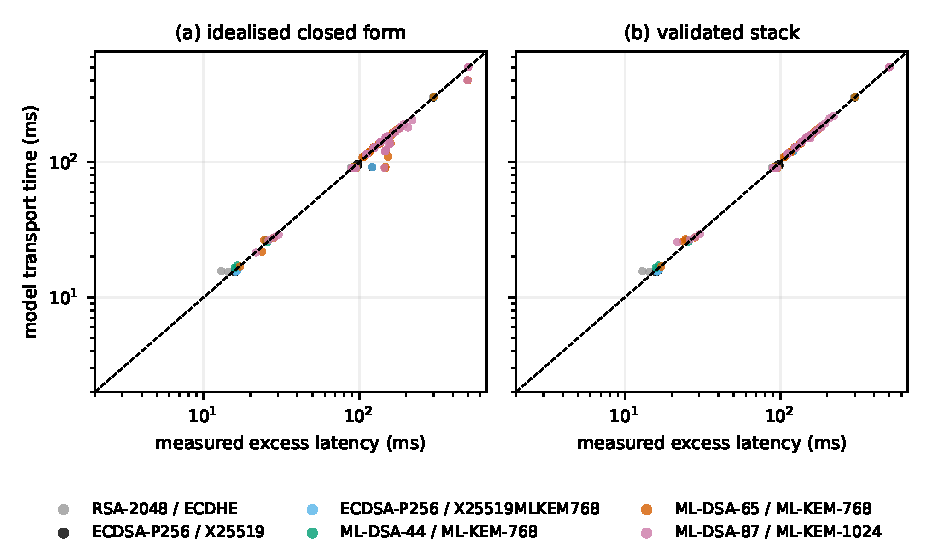
\includegraphics[width=\textwidth]{figures/fig_testbed}
\caption{Measured excess latency against the model for \tbNConfigs\ configurations: (a)~idealised closed form, (b)~model with Linux window validation and the OpenSSL write pattern. The points far below the diagonal in (a) are whole-round-trip errors.}
\label{fig:testbed}
\end{figure}

\begin{table}[t]
\centering\small
\caption{Mean absolute error of the model against the testbed (ms), per suite (signature and key-exchange pair).}
\label{tab:testbed}
\begin{tabular}{@{}>{\raggedright\arraybackslash}p{0.30\textwidth}rrrr@{}}
\toprule
\shortstack[l]{Signature /\\key exchange} & \shortstack[r]{Config-\\urations} & \shortstack[r]{MAE ideal\\(ms)} & \shortstack[r]{MAE stack\\(ms)} & \shortstack[r]{Within\\1\,ms} \\
\midrule
RSA-2048 / ECDHE & 12 & 0.95 & 0.95 & 6 of 12 \\
ECDSA-P256 / X25519 & 63 & 1.96 & 1.48 & 36 of 63 \\
ECDSA-P256 / X25519MLKEM768 & 15 & 2.59 & 0.64 & 15 of 15 \\
ML-DSA-44 / ML-KEM-768 & 12 & 0.66 & 0.72 & 9 of 12 \\
ML-DSA-65 / ML-KEM-768 & 62 & 7.02 & 1.89 & 23 of 62 \\
ML-DSA-87 / ML-KEM-1024 & 62 & 7.18 & 2.14 & 21 of 62 \\
\midrule
All & 226 & 4.70 & 1.65 & 110 of 226 \\
\bottomrule
\end{tabular}

\end{table}

\subsection{Middlebox penalty}
The model needs the penalty $\pi$ per flight longer than $\theta$ segments only if a middlebox delays long flights. On the direct path, the least-squares fit gives $\pi=\tbPiFit$\ms at $\theta=\tbThetaFit$ segments, with a root-mean-square error of $\tbRmseBestPi$\ms against $\tbRmseZeroPi$\ms at $\pi=0$: no penalty is needed. We then inserted HAProxy~2.8 as a TCP proxy between the two namespaces, either forwarding bytes as they arrive or waiting for the complete ClientHello before routing. Over \tbProxyTcpN\ configurations (the suites ECDSA-P256, ML-DSA-44, ML-DSA-65 and ML-DSA-87 at chain depths 1 to 4, 30\ms RTT, 100\,Mbit/s, MTU 1500, initial window 10, with flights of 2 to 27 segments), the proxy added on average \tbProxyTcpMean\ms (range \tbProxyTcpLo\ to \tbProxyTcpHi\ms) in the first mode and \tbProxyInspectMean\ms (\tbProxyInspectLo\ to \tbProxyInspectHi\ms) in the second, independently of the flight size. This is a check of one proxy, one version and one configuration, not a statement about proxies in general. The values of $\pi$ up to 24\ms swept in this paper therefore stand for devices that we did not test, such as deep packet inspection, TLS-terminating proxies or hardware firewalls; $\pi=0$ is the value supported by the measurements and is used for the single values reported below.

\section{Results}
\label{sec:results}

RQ1 was answered in \cref{sec:testbed}; the results below use the model validated there. \Cref{tab:master} summarises the answers to RQ2--RQ5 for every suite; the following subsections explain the underlying mechanisms, and \cref{sec:sens,sec:rq5} test how far they depend on the model inputs (RQ6).


\begin{table}[t]
\centering\small
\caption{Summary of results per suite. RQ2: cold SWIFT~MX transaction at depth 3. RQ3: latency added from depth 1 to 4 (SWIFT~MX). RQ4: share of cold configurations in which the transport overhead $O$ exceeds cryptographic time. RQ5: certificate bytes removed by compression. RQ6 is answered by the uncertainty analysis in \cref{sec:rq5}.}
\label{tab:master}
\resizebox{\textwidth}{!}{\begin{tabular}{@{}lrrrr@{}}
\toprule
Suite & RQ2: size, KB & RQ3: $\Delta T_{d1\to d4}$ & RQ4: $O>T_\text{cpu}$ & RQ5: cert.\ bytes \\
 & (factor) & (ms) & (\% of configs) & compressed (\%) \\
\midrule
RSA-2048 & 27.2 (1.2$\times$) & 0.6 & 45 & 22 \\
RSA-3072 & 30.0 (1.3$\times$) & 0.9 & 44 & 18 \\
ECDSA-P256 (baseline) & 23.0 (1.0$\times$) & 29.6 & 51 & 31 \\
ECDSA-P256 + hybrid KEM & 25.2 (1.1$\times$) & 29.6 & 56 & 31 \\
ML-DSA-44 & 66.3 (2.9$\times$) & 31.4 & 84 & 6 \\
ML-DSA-65 & 83.4 (3.6$\times$) & 60.0 & 87 & 5 \\
ML-DSA-87 & 106.8 (4.6$\times$) & 32.3 & 93 & 3 \\
Falcon-512 & 39.9 (1.7$\times$) & 1.2 & 80 & 12 \\
Falcon-1024 & 56.4 (2.4$\times$) & 30.9 & 85 & 7 \\
SLH-DSA-128s & 126.3 (5.5$\times$) & 32.7 & 0 & 3 \\
SLH-DSA-128f & 246.7 (10.7$\times$) & 64.9 & 84 & 2 \\
ML-DSA-44+ECDSA-P256 & 67.9 (2.9$\times$) & 31.7 & 84 & 6 \\
ML-DSA-65+ECDSA-P256 & 84.9 (3.7$\times$) & 60.4 & 85 & 4 \\
\bottomrule
\end{tabular}
}
\end{table}

\subsection{RQ2: The security envelope dominates transaction size}
ML-DSA-65 with ML-KEM-768 enlarges a cold SWIFT~MX transaction from \swiftKBbase\ to \swiftKBMLDSAsixtyfive\KB; Falcon-512 brings it to \swiftKBFalconFiveTwelve\KB and SLH-DSA-128f to \swiftKBSLHf\KB (\cref{fig:sizes}). For ML-DSA-65, certificate chains account for $\swiftMLcertShare\%$ of the bytes, signatures and embedded certificates in XMLDSig for $\swiftMLappShare\%$, \texttt{CertificateVerify} for $\swiftMLcvShare\%$, and the payment payload for only $\swiftMLfixedShare\%$. Lean protocols grow most: ISO~8583 grows $\xISOEightFiveEightThreeMLDSAsixtyfive\times$ with ML-DSA-65 because its handshake chains dwarf a 300-byte authorisation, against $\xISOTwoZeroZeroTwoTwoMLDSAsixtyfive\times$ for ISO~20022 and $\xFAPITwoMLDSAsixtyfive\times$ for FAPI~2.0 (\supp{Table S3}). The hybrid key share adds only \hybridDeltaKB\KB. On a warm connection, ISO~8583 is unaffected (symmetric MAC), whereas ISO~20022 still grows $\warmXIsoTwoZeroTwoTwo\times$ and FAPI~2.0 $\warmXFAPITwo\times$ because of application-layer signatures.

\begin{figure}[t]
\centering
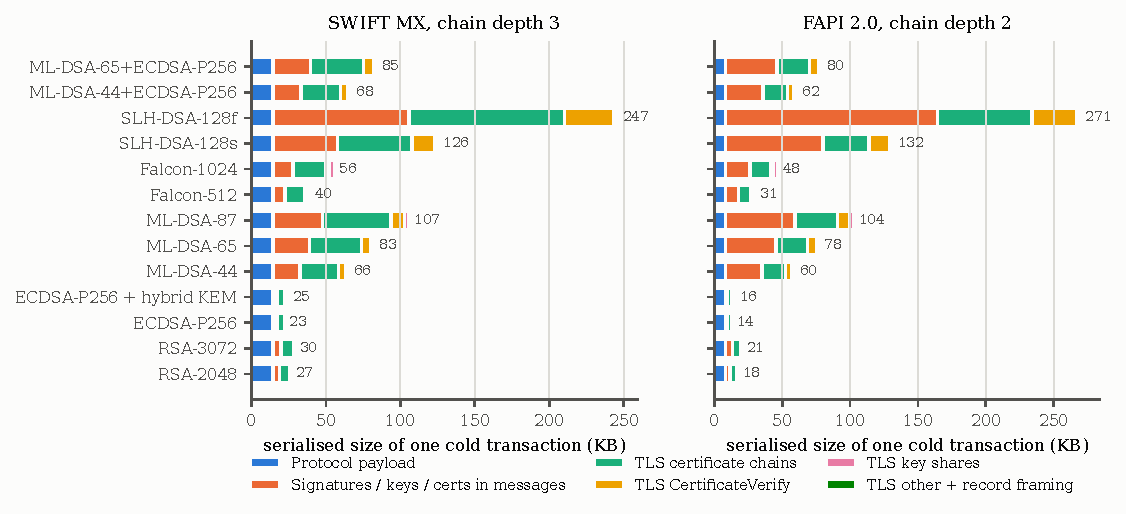
\includegraphics[width=\textwidth]{figures/fig_sizes}
\caption{Composition of a cold transaction: SWIFT~MX at depth 3 (left) and FAPI~2.0 at depth 2 (right). Totals in KB.}
\label{fig:sizes}
\end{figure}

\subsection{RQ3: Latency grows in round-trip steps}
\Cref{fig:depth} shows SWIFT~MX latency against chain depth: it grows in whole round trips. The classical baseline gains $+\ecDepthDelta$\ms from depth 1 to 4, one round trip, because from depth 2 the client flight (a handshake flight and the request of about 11\KB, written separately) no longer fits the initial window of ten segments; ML-DSA-65 gains $+\mlDepthDelta$\ms, two round trips, of which $\mlDepthSsw$\ms are slow-start waits, $\mlDepthSer$\ms serialisation and $\mlDepthCpu$\ms computation. The post-quantum-specific cost of three additional certificates is the difference, $\mlDepthNet$\ms or about $\perCertNet$\ms per certificate (an average: the baseline pays its round trip at one depth, not gradually), against $\perCertOneFiveZeroZeropZero$\ms in absolute terms at MTU 1500 ($\perCertRttFive$\ms at 5\ms RTT, $\perCertRttOneZeroZero$\ms at 100\ms). Jumbo frames cut it to $\perCertNineZeroZeroZeropZero$\ms, a transport penalty of 24\ms would raise it to $\perCertNineZeroZeroZeropTwoFour$\ms (\supp{Tables S4--S6}), and an initial window of 32 segments halves the depth effect ($+\icwThirtyTwoMLDelta$\ms).

Where a flight lands depends on the stack (\cref{sec:testbed}). An idealised closed form would make the hybrid suite faster than the baseline at MTU 1280 ($\hybKneeHybIdeal$ vs.\ $\hybKneeBaseIdeal$\ms), the composite suite $+\compositeDepthDeltaIdeal$\ms against $+\mlDepthDeltaIdeal$\ms for ML-DSA-65, and the classical baseline flat ($+\ecDepthDeltaIdeal$\ms); these are artefacts. With the validated stack the hybrid suite is not faster ($\hybKneeHyb$ vs.\ $\hybKneeBase$\ms; measured \tbKneeHyb\ vs.\ \tbKneeBase\ms on SWIFT-sized transactions), the composite suite behaves like ML-DSA-65 ($+\compositeDepthDelta$ vs.\ $+\mlDepthDelta$\ms) and the baseline pays one round trip. ML-DSA-87 shows a smaller depth effect than ML-DSA-65 ($+\mlDepthDeltaEightSeven$ vs.\ $+\mlDepthDelta$\ms) in both variants, because its flights already cross an additional window boundary at depth~1. The gap between post-quantum and classical suites does not depend on these details (\cref{sec:sens}).

\begin{figure}[t]
\centering
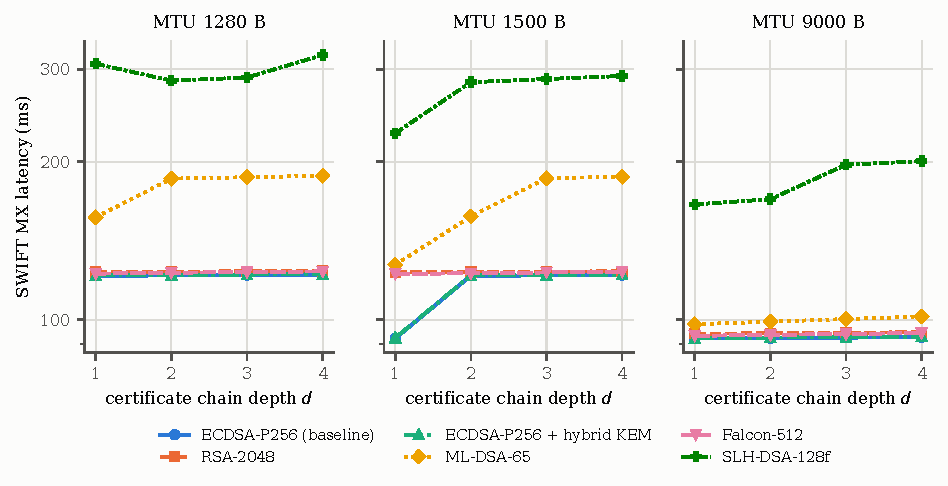
\includegraphics[width=\textwidth]{figures/fig_depth}
\caption{SWIFT~MX latency against chain depth for three MTUs (100\,Mbps, 30\ms RTT, no penalty; log scale).}
\label{fig:depth}
\end{figure}

\subsection{RQ4: Transport, not cryptography, sets the cost}
Transport overhead exceeds cryptographic time in $\shareECxOne\%$ of the configurations even for the classical baseline, and in $\shareMLxOne\%$ for ML-DSA-65 (\cref{tab:master}); these shares are fractions of the evaluated parameter grid, which weights every combination equally, and not of the transactions of any bank; for ML-DSA-65 the share remains $\shareMLxOneSix\%$ with sixteen-fold slower cryptography. With the costs measured on the x86 core the shares are $\cpuShareMl\%$ for ML-DSA-65, $\cpuShareFal\%$ for Falcon-512 and $\cpuShareEc\%$ for the baseline, close to those of a four-fold scale ($\shareMLxFour\%$, $\shareFalxFour\%$ and $\shareECxFour\%$). The model adds the computation of the steps serially, so $T_\text{cpu}$ is the sum of the primitive costs in protocol order and not a measurement of the CPU time that blocks the critical path. The following overlap scenarios are assumptions, not measurements: if part of the computation overlapped with the network, so that only half or a quarter stayed on the critical path, the shares would rise to $\shareMLxHalf\%$ and $\shareMLxQuarter\%$ for ML-DSA-65 and to $\shareECxHalf\%$ and $\shareECxQuarter\%$ for the baseline, so the conclusion about the dominance of transport depends on this assumption only in being conservative with respect to it (SLH-DSA-128s, which is bound by computation, is the exception: $\shareSLHsxHalf\%$ at half). The post-quantum penalty is therefore almost entirely a change in the transport term, not in computation: for the lattice schemes, the added overhead exceeds the added cryptographic time in most configurations (\supp{Table S9}). \Cref{fig:ratio} shows that the ratio barely depends on bandwidth above 100\,Mbps, because the slow-start wait depends on the RTT and the flight size rather than on bandwidth. The exception is SLH-DSA-128s, whose four signatures cost \slhsCpuMs\ms per SWIFT~MX transaction and outweigh transport in every configuration; SLH-DSA-128f, by contrast, is transport-bound because of its 17-KB signatures.

\begin{figure}[t]
\centering
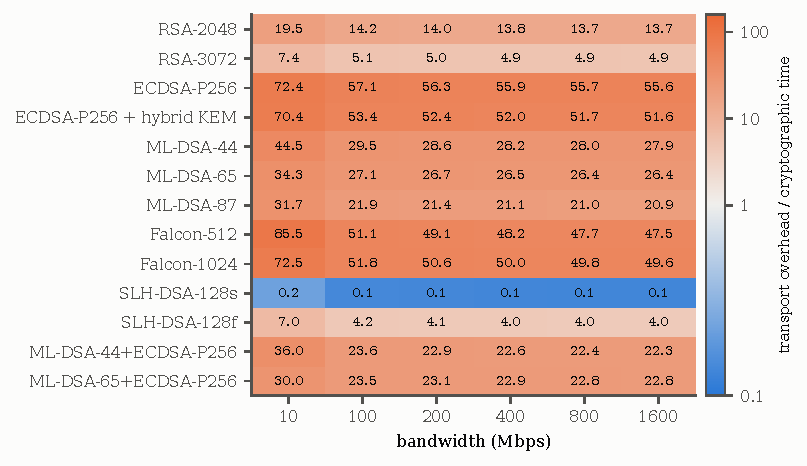
\includegraphics[width=0.7\textwidth]{figures/fig_ratio}
\caption{Ratio of transport overhead $O$ to cryptographic time (SWIFT~MX, depth 3, 30\ms RTT, MTU 1500). Orange cells: transport dominates.}
\label{fig:ratio}
\end{figure}

\subsection{RQ5: Certificate compression rarely helps post-quantum chains}
Because keys and signatures are pseudorandom, compression removes $\ccRedEC\%$ of an ECDSA-P256 chain but only $\ccRedML\%$ of an ML-DSA-65 chain. It saves at least 1\ms in only $\ccMatLo$--$\ccMatHi\%$ of configurations, and the saving is essentially binary---zero or one RTT---depending on whether a flight drops below a window boundary. Decompression can cost more than it saves: with an embedded client inflating at 3.3\,MB/s, compression is net-harmful in $\harmEmbML\%$ of ML-DSA-65 configurations, against $\harmEmbEC\%$ for ECDSA-P256, and the median break-even speed for ML-DSA-65 is about \beMLmbs\,MB/s (\supp{Table S7, Fig.~S1}). Real chains confirm the premise: zlib at level 9 reduces real ML-DSA and SLH-DSA chains only to $\compRealPQlo$--$\compRealPQhi$ of their size, within $\compErrPQ\%$ of the model (\supp{Table S13}).


\subsection{Sensitivity to model inputs}
\label{sec:sens}
We varied the certificate metadata (600--1\,400\,B per leaf), XMLDSig certificate embedding, the window of reused connections (\supp{Table S8}). Omitting the signer certificate from XMLDSig reduces the ML-DSA-65 SWIFT~MX transaction from \swiftKBMLDSAsixtyfive\ to \nocertMLKB\KB. A reused connection that keeps a large window ($c=64$) reduces the warm ML-DSA-65 ISO~20022 exchange from \idleWarmML\ to \busyWarmML\ms (baseline: \busyWarmBase\ms). Individual steps move with these parameters, but the ranking Falcon-512 $<$ ML-DSA $<$ SLH-DSA-128f, with SLH-DSA-128s bound by computation, holds in every variant. A variance-based global sensitivity analysis over the full factorial designs (first- and second-order indices, \supp{Table S17}) shows that the round-trip time explains $\sobolLatRtt$ of the variance of log latency and the suite $\sobolLatSuite$, while the post-quantum \emph{factor} of the lattice schemes is governed by the MTU ($\sobolLatMtu$), the RTT ($\sobolLatRttF$) and the suite ($\sobolLatSuiteF$).

\subsection{RQ6: Robustness to parameters that nothing fixes}
\label{sec:rq5}
The wired model is deterministic, so the only uncertainty is in inputs that no standard or measurement fixes. We drew the certificate metadata (600--1\,400\,B per leaf, with CA metadata moving with it), the CPU scale (log-uniform 1--16$\times$, i.e.\ from the measured core to a hardware security module or constrained device), the penalty $\pi$ (0--24\ms), the threshold $\theta$ (2--16 segments) and the initial window (10, 32 or 64 segments with probability 0.6, 0.3 and 0.1) 4\,000 times and recomputed a SWIFT~MX transaction at depth 2, 100\,Mbps, 30\ms RTT (\supp{Table S18}). These priors are our assumptions, not fitted distributions, so the intervals below are conditional on them (an assumption-based uncertainty analysis) and are not confidence intervals of the performance of any bank; they also leave out structural uncertainty (other operating systems, TLS libraries and middleboxes, jitter and loss, the traffic of individual institutions). The ranking Falcon-512 $<$ ML-DSA-65 $<$ SLH-DSA-128f holds in $\uOrderHolds\%$ of the draws, and transport overhead exceeds cryptographic time in $\uOverheadShare\%$ of them ($\uOverheadLowCpu\%$ for CPU scales below 4, $\uOverheadHighCpu\%$ between 12 and 16). The ML-DSA-65 factor has a median of $\uMlFactorMed$ (90\% interval $\uMlFactorLo$--$\uMlFactorHi$) and Falcon-512 of $\uFalFactorMed$ ($\uFalFactorLo$--$\uFalFactorHi$). For the factor, the CPU scale ($\rho=\uRhoCpuFactor$) and the penalty $\pi$ ($\rho=\uRhoPenFactor$) matter more than the initial window ($\rho=\uRhoCwndFactor$); for the cost per additional certificate the initial window dominates ($\rho=\uRhoCwndPerCert$). In particular, the figure of about 20\ms per additional ML-DSA-65 certificate holds for the default window of 10 segments (median $\uPerCertWTenMed$\ms, 90\% interval $\uPerCertWTenLo$--$\uPerCertWTenHi$\ms); with 32 segments it is $\uPerCertWThirtyTwoMed$\ms ($\uPerCertWThirtyTwoLo$--$\uPerCertWThirtyTwoHi$) and with 64 segments $\uPerCertWSixtyFourMed$\ms ($\uPerCertWSixtyFourLo$--$\uPerCertWSixtyFourHi$). The headline cost is therefore an upper estimate for servers that raise the initial window. Because the testbed found no penalty for a TCP proxy (\cref{sec:testbed}), the upper part of the factor intervals applies only to devices that we did not test.

\section{Discussion}
\label{sec:discussion}

\subsection{What the results mean}
The results agree with handshake-level measurements in which Falcon-512 is the only post-quantum scheme whose server flight fits in a single packet~\cite{raavi2025}, and with field measurements in which 17\KB of additional handshake data, the size of a Dilithium2 drop-in, slows the median handshake by about 20\%~\cite{westerbaan2021}. They add five points that matter for financial systems.

\emph{First}, the stack decides where the round trips fall. A flight costs an extra round trip only if it does not fit in the congestion window, and whether it fits is not a function of its size alone: it depends on how many segments the writes of the TLS library produce (the 4\,096-byte handshake buffer of OpenSSL and the separate request write add one to three segments per transaction) and on how the kernel grows the window (Linux does not enlarge it after a short flight such as the ClientHello). A closed form that ignores both is off by more than 0.4 round trips in \tbOffIdeal\ of \tbNConfigs\ configurations and produces effects that do not occur, such as a hybrid suite that is faster than the baseline (\cref{sec:testbed}). For practitioners this means that the number of round trips of a post-quantum migration cannot be read off message sizes: it has to be established on the deployed stack, and a change as small as the position of the request write can move a flight across the window boundary.

\emph{Second}, the penalty is a round-trip effect. For ML-DSA-65, a chain that grows from depth~1 to 4 adds $\mlDepthDelta$\ms to a SWIFT~MX transaction at 100\,Mbps and 30\ms RTT, of which $\mlDepthSsw$\ms are slow-start waits and only $\mlDepthCpu$\ms computation; the classical baseline gains $\ecDepthDelta$\ms, one round trip, so that the post-quantum-specific cost is $\mlDepthNet$\ms. Each extra ML-DSA-65 certificate costs about two thirds of an RTT ($\perCertRttFive$\ms at 5\ms, $\perCertRttOneZeroZero$\ms at 100\ms), which is why the cost cannot be recovered by faster hardware: transport overhead exceeds cryptographic time in $\shareMLxOne\%$ of the evaluated ML-DSA-65 configurations and still in $\shareMLxOneSix\%$ when cryptography is sixteen times slower.

\emph{Third}, the cost is an architectural decision. Certificate chains account for $\swiftMLcertShare\%$ of the bytes of an ML-DSA-65 SWIFT~MX transaction and the signatures embedded in XMLDSig for another $\swiftMLappShare\%$, so chain depth and the choice to embed the signer certificate matter as much as the algorithm: referencing instead of embedding the certificate reduces the transaction from \swiftKBMLDSAsixtyfive\ to \nocertMLKB\KB. With a chain of two intermediates, an ML-DSA-65 server flight is several times the 4\KB or less that most TLS connections send today~\cite{kampanakis2022}.

\emph{Fourth}, the same mechanism applies to application-layer signatures whenever a connection starts, or restarts after idling, from the initial window. Keeping a window open on a reused connection reduces a warm ML-DSA-65 ISO~20022 exchange from \idleWarmML\ to \busyWarmML\ms (baseline \busyWarmBase\ms), and an initial window of 32 segments halves the depth effect ($\mlDepthDelta\to\icwThirtyTwoMLDelta$\ms), but the second is only possible on paths that an operator controls.

\emph{Fifth}, the choice of signature should follow the role. Falcon-512 enlarges a SWIFT~MX transaction $\swiftXFalconFiveTwelve\times$ against $\swiftXMLDSAsixtyfive\times$ for ML-DSA-65; SLH-DSA-128s costs \slhsCpuMs\ms of computation per transaction and SLH-DSA-128f \swiftKBSLHf\KB of bytes, so hash-based schemes belong to roots and offline signing and not to interactive paths. These are performance rankings: Falcon-512 is the cheapest in transport, but whether it can be deployed depends on its standardisation status, on support in libraries and hardware security modules and on interoperability, none of which this study assesses. \supp{Table S22} gives the standardisation status on 31 October 2026: FIPS 204 and 205 and the X.509 profiles of ML-DSA and SLH-DSA (RFC~9881, RFC~9909) are final and the TLS signature schemes for ML-DSA are in the RFC Editor queue, whereas FIPS 206 (Falcon) is still in development and the composite scheme is still an Internet-Draft. Vendors have announced algorithm validations of ML-DSA, ML-KEM and SLH-DSA in hardware security modules, but we did not assess any of them. Certificate compression is not a remedy: it removes $\ccRedML\%$ of an ML-DSA-65 chain against $\ccRedEC\%$ of an ECDSA chain and is harmful on slow clients.

\subsection{Guidance}
Within the scope of a wired path, the results support the following checklist, in order of effect: (i)~count the segments and round trips of the deployed stack (write pattern of the TLS library, window behaviour of the kernel, kernel TCP counters) instead of inferring them from message sizes; (ii)~keep chains shallow ($d\le2$) and never send roots; (iii)~reference rather than embed certificates in XMLDSig; (iv)~reuse connections and keep windows open; (v)~use compact signatures on online paths and keep SLH-DSA offline; (vi)~do not rely on certificate compression; (vii)~where the path is controlled, raise the initial window and the MTU, which is the single most effective lever (the median cost per certificate falls from $\uPerCertWTenMed$\ms to $\uPerCertWThirtyTwoMed$\ms at 32 segments, \cref{sec:rq5}). Techniques that shorten the handshake itself (session resumption, cached or Merkle-tree chains, QUIC) and the cost on mobile access are outside the scope of this study.

\subsection{Limitations}
The reported latencies are model outputs driven by measured inputs. They were validated on one stack: Linux TCP with Reno and quick acknowledgements, OpenSSL~3.5, one pair of cores, one middlebox type (HAProxy) and a wired emulated link, without the jitter, loss and queueing of a real wide-area path. The two stack behaviours that the model needs, the window validation of Linux and the write pattern of OpenSSL, were observed on Linux 7.0 and OpenSSL~3.5.4 and are specific to this stack (we did not test other kernel versions or other TLS libraries, and BBR lies outside the model): other TLS libraries write handshakes differently and other operating systems grow the window differently, and either would move individual flights across a window boundary; a different stack changes where the round trips fall, not the order of the schemes. \chg{The testbed and the model use full handshakes without session tickets, whereas production servers issue them. In a follow-up experiment (data in the artefact repository from its next release) a full transaction that also issued one ticket was slower than the ticketless one by half a round trip in six of 40 configurations (ECDSA at chain depth three, ML-DSA at depth one, MTU 1500) and equal in the others, so the full-handshake latencies reported here may be up to half a round trip too low where tickets are issued; the model has no mode for it (Table S23 of the Supplementary Material).} The profiles are representative models: ISO~20022 and SWIFT~MX messages are signed with XMLDSig that embeds the signer certificate by default in our model, which is a modelling choice and not a requirement of these standards (institutions may use MACs, other envelopes or certificate references; the effect of referencing is reported in \cref{sec:sens}), and message sizes are typical values rather than institutional traces. The testbed covers the rates, MTUs and initial windows listed in \cref{sec:testbed} and, at 100\,Mbit/s, CUBIC, delayed acknowledgements and timestamps; the rest of the parameter grid, in particular loss, bandwidths above 1\,Gbit/s and round-trip times other than 5, 30 and 100\ms, is extrapolated by the model. CPU costs were measured on one Arm platform and one x86 core (an older laptop core) and depend on the implementation (ML-DSA-65 signing differs by a factor of two between OpenSSL and liboqs); the factor 4 agrees with the x86 measurement, but the factor 16 for hardware security modules and constrained devices is an assumption, not a measurement. \chg{A direct measurement of an event-driven OpenSSL server on one Cortex-X925 core (loopback, Table S24 of the Supplementary Material) puts the CPU per handshake at \srvPqOvhMin{}--\srvPqOvhMax{} times the primitive costs of the model for the post-quantum and RSA suites and at \srvEcOvhMin{}--\srvEcOvhMax{} times for the classical ECDSA suites, because TLS, the kernel and the event loop add a few tenths of a millisecond per handshake; these ratios lie within the CPU scales of 1 to 16 times swept here.} The one operational test of post-quantum signatures in a payment system that we know of reports a verification time of 209.9\ms on the receiving side, about three orders of magnitude above the 0.1--0.3\ms that we measure for ML-DSA-65 verification (\supp{Table S19}); the report does not say what the verification step contains (message queues, a Java runtime, the middleware around the cryptographic library)~\cite{bis_leap2025}. The cost of integrating message-level verification into an operational system can therefore exceed the cost of the primitive by far, and our CPU scales of 1--16$\times$ do not cover it: our finding that transport overhead exceeds cryptographic time concerns the primitives and the TLS and XMLDSig operations that we model, not the processing of a payment system behind its gateway. Message sizes are representative values rather than institutional traces, and the certificate chains of financial networks are not public, so the depth effect is reported per certificate. SLH-DSA and Falcon could not be exercised in TLS because OpenSSL~3.5 has no code points for them. The penalty $\pi$ was measured only for a TCP proxy; deep packet inspection and hardware firewalls were not tested, and a field experiment in which connections drop at handshake sizes of about 10\KB and 30\KB~\cite{westerbaan2021} shows that real middleboxes can fail and not only delay. The wired model has no receive-window limit, and packet loss was neither measured on the testbed nor modelled with the validated stack: an earlier simulation with the idealised segmentation is in the repository but is not used in this paper. Individual round-trip steps are discrete, so single configurations should not be over-interpreted, whereas aggregate shares, factors and rankings held in all sensitivity variants.

%% ============================================================================================
\section{Conclusion}
\label{sec:conclusion}
The cost of post-quantum signatures in financial messaging is not a function of message size alone: it is paid in round trips, and the transport stack decides where they fall. Linux enlarges the congestion window only while it is below twice the segments in flight, and OpenSSL writes a handshake through a 4\,096-byte buffer with the request as a separate write; a model that includes these two behaviours reproduces \tbNTrans\ OpenSSL transactions over a kernel-emulated link to within \tbMaeStack\ms on average, whereas an idealised closed form errs by \tbMaeIdeal\ms and by whole round trips. For lattice-based signatures, post-quantum migration changes the transport behaviour of banking transactions far more than their computation. Larger keys and signatures turn into extra segments and, above all, extra round trips when flights outgrow the congestion window; the cost therefore scales with the round-trip time and with the depth of the certificate chains of both peers, and it is largely independent of CPU speed. A closed-form transport model, calibrated on measured CPU costs and validated against real OpenSSL~3.5 handshakes, certificates and signed objects and against an independent discrete-event implementation, predicts these effects over $\nConfigs$ configurations. Compact signatures, shallow chains, referenced rather than embedded certificates and reused connections are the effective levers on a wired path, whereas zlib certificate compression helps little in the configuration tested. The artefacts of an idealised closed form (a faster hybrid suite, a flat classical baseline) do not occur on real transactions, an HAProxy TCP proxy adds no measurable penalty in the configurations tested, and other TLS stacks, deep packet inspection and real wide-area paths remain to be measured.

\section*{Data availability}
The simulator, the independent discrete-event cross-check, the measurement and testbed scripts, the raw testbed measurements (\tbNTrans\ transactions), the x86 and Arm CPU measurements, the unit tests and the scripts that generate every table, figure and number of this paper are available at \url{https://github.com/tronghieudinh/pqc-financial-transport} and archived at Zenodo (version \texttt{paper1-v1.2} used for this paper~\cite{dinh2026artifact}; the DOI \href{https://doi.org/10.5281/zenodo.23839449}{10.5281/zenodo.23839449} always resolves to the latest version). The simulation results (about 260\,MB) are regenerated in under a minute by \texttt{reproduce.sh}. The test private keys of the generated certificate chains are not distributed; \texttt{certs.sh} regenerates them. The institutional message traces and certificate chains of financial networks are not public and were not used.

\section*{Declarations}
\textbf{CRediT authorship contribution statement:}

\textbf{Trong-Hieu Dinh:} Conceptualization, Methodology, Software, Investigation, Formal analysis, Data curation, Visualization, Writing -- original draft, Writing -- review \& editing.
\textbf{Trong-Minh Hoang:} Supervision, Resources, Formal analysis, Writing -- review \& editing.


\textbf{Declaration of competing interest:}  The authors declare\ no known competing financial interests or personal relationships that could have appeared to influence the work reported in this paper.

%\textbf{Funding:} This research did not receive any specific grant from funding agencies in the public, commercial, or not-for-profit sectors.

\section*{Declaration of generative AI and AI-assisted technologies in the manuscript preparation process}
During the preparation of this work  T.-H. Dinh\ used Claude (Anthropic) in order to develop simulation and analysis code, to draft and edit text, and to check numbers against the data. After using this tool,  the authors reviewed and edited the content as needed and take\ full responsibility for the content of the publication.

\bibliographystyle{elsarticle-num}
\bibliography{refs}
\end{document}
